% !TeX root = ../../Book3.tex
% 纲要标题：## 第23章　Plateau 问题与变分流形
% 纲要位置：几何学计划纲要.md，第 3071 行。
% 正文状态：初稿；尚未正式审核。

% 纲要内容开始
% 
% > 本章目标与证明范围：在给定可填充的紧支整数边界和质量有限的竞争类中，完整证明欧氏 Plateau 存在性。存在性、内部正则性、边界正则性及弱模型选择分开；一般奇异集界逐版本外引。
% 
% 纲要内容结束

\chapter{Plateau 问题与变分流形}
\label{g3:ch:23}
\BookChapterNumber{g3:ch:23}

\begin{chapterabstract}
	给定整数边界后，面积极小化首先需要一个能容纳极限的竞争类。本章在全部有限质量整数流中完整证明 Euclid 空间的 Plateau 存在性：锥保证非空，凸投影给出共同紧支集，整数流紧性、边界连续性与质量下半连续性产生极小解。随后推导驻值性、单调性和密度公式，结合准确列出的外部紧性与正则性结果讨论切锥、内部奇点和边界几何。变分流形以位置及无取向切平面上的正测度保存面积，适合描述驻值极限。最后用离散短测地线替换完整证明黎曼二球面上非平凡闭测地线的存在，并在指定系数、拓扑和维数下陈述 Almgren--Pitts 极小超曲面存在性及指标结论。
\end{chapterabstract}

\begin{learninggoals}
	\begin{itemize}
		\item 准确写出给定整数边界的竞争类，检验非空性以及零维边界的总系数条件。
		\item 用最近点投影控制支集，逐项完成极小化序列、整数极限与最小值的证明。
		\item 以校准计算填充质量，利用消失分支和细把手辨别边界约束与拓扑约束。
		\item 推导流的驻值公式、面积单调性及密度下界，理解切锥构造对质量收敛的需要。
		\item 区分密度一正则性、高重数分支、内部奇异集界及边界正则性的条件。
		\item 定义变分流形，计算推前、第一变分、广义平均曲率和边界力，并核验 Allard 定理的输入。
		\item 由度为一的扫掠、正宽度和偶奇短线替换构造非恒定闭测地线。
		\item 在超曲面极小极大问题中分别说明系数、收敛拓扑、重数、支集正则性与指标。
	\end{itemize}
\end{learninggoals}

一条平面圆周张成的圆盘有一个直接的面积下界：将任何候选曲面投影回圆周所在平面，投影面积不能增加，而有向边界仍是原圆周。对于一般空间闭曲线，未必能立即写出最小曲面，但同样可以先把所有候选者放进一个有紧性的类，再让面积趋于下确界。Plateau 问题\footnote{Joseph Antoine Ferdinand Plateau（1801--1883），比利时物理学家，研究视觉现象、毛细作用与液膜的平衡形状。}由此把几何中的面积比较变成了一个关于弱极限的存在性问题。

\ProseParagraphBreak
第22章已经证明：共同紧支且质量、边界质量有界的整数流列，有整数流的平坦收敛子列。现在需要把这项工具接到一个具体极小化问题上。给定的边界是否能够填充？竞争者能否逃向无穷远？极限是否还具有同一个有向边界？本章的前两节逐一解决这些问题，并保留竞争类中真正写出的条件。

\ProseParagraphBreak
存在的极小流还需要几何解释。对它作径向变形，可以比较不同半径内的质量；放大观察得到的切锥则显示密度和重数。一张平面作为切锥并不总意味着原对象光滑：复曲线的分支点可以具有重数二的平面切锥。内部正则性与边界正则性因此分别按维数、余维、重数及边界条件陈述。

\ProseParagraphBreak
最后两节转向面积驻值的另一种描述。流会记录取向抵消，变分流形则把各层面积保存在正测度中。后者可以承接一族曲面的极小极大过程。作为能够在本章直接完成的模型，我们用短弧替换构造二球面上的闭测地线；高维极小超曲面的构造则准确调用所选的 Almgren--Pitts 版本。前两节依赖第22章的推前、锥、紧性与质量下半连续性；密度分析使用第20章的面积与可整流密度结果，扫掠曲线还使用第6章的短测地线和能量比较，以及第二卷已经建立的映射度。

% !TeX root = ../../Book3.tex
% 纲要标题：### 23.1 Plateau 问题的竞争类
% 纲要位置：几何学计划纲要.md，第 3075 行。
% 正文状态：初稿；尚未正式审核。

% 纲要内容开始
% 
% * 边界流、竞争类和非空性
% * 锥构造与初始填充
% * 凸投影控制支集
% * 极小化序列及质量界
% 
% 纲要内容结束

\section{Plateau 问题的竞争类}
\label{g3:sec:2301}
固定一条空间闭曲线后，“寻找面积最小的曲面”还没有指定一个变分问题：允许哪些曲面，怎样理解边界，是否固定拓扑类型，都需要说明。这里用整数流记录取向、重数与边界，用质量作为面积。第22章已经给出这个类的紧性；本节补上竞争类非空以及极小化序列不向无穷远逃逸的条件。

\subsection{边界流、竞争类和非空性}
\label{g3:subsec:2301:01}
设 \(1\le k\le n\)，给定紧支整数 \((k-1)\) 流 \(B\in\mathcal I_{k-1}(\mathbb R^n)\)。我们寻找满足 \(\partial T=B\) 的整数 \(k\) 流。下标 \(k\) 是待求对象的维数；通常的空间曲线张成曲面问题对应 \(k=2,n=3\)。

\begin{definition}\label{g3:def:plateau-competitor-class}
	对紧支 \(B\in\mathcal I_{k-1}(\mathbb R^n)\)，定义竞争类及其质量下确界
	\begin{equation}\label{g3:eq:plateau-competitor-class}
		\mathcal A(B)=\{T\in\mathcal I_k(\mathbb R^n):\partial T=B\},
		\qquad m(B)=\inf_{T\in\mathcal A(B)}\mathbf M(T).
	\end{equation}
	空类的下确界约定为 \(+\infty\)。若 \(\mathcal A(B)\ne\varnothing\)，称 \(B\) 可填充。求取达到 \(m(B)\) 的元素，称为这里的\term[zhengshu liu Plateau wenti]{整数流 Plateau 问题}[integral-current Plateau problem]。
\end{definition}

\(\mathcal I_k\) 已要求流及其边界的总质量有限。因此所有竞争者都满足 \(\mathbf M(T)<\infty\)，且边界质量固定为 \(\mathbf M(B)\)。定义暂不要求竞争者紧支；允许的拓扑类型、连通分支数和整数重数也未另加限制。若把“参数域为一个圆盘”或“承载集必须连通”写入定义，得到的便是另一个竞争类，需要另行证明它在所选收敛下保持。

\begin{proposition}\label{g3:prop:euclidean-fillability}
	设 \(1\le k\le n\)，\(B\in\mathcal I_{k-1}(\mathbb R^n)\) 紧支。若 \(k\ge2\)，则 \(\mathcal A(B)\ne\varnothing\) 当且仅当 \(\partial B=0\)。若 \(k=1\)，则 \(\mathcal A(B)\ne\varnothing\) 当且仅当 \(B(1)=0\)，其中 \(B(1)\) 表示有限个带整数权点的总系数。在这两种情形下，非空类中都有紧支元素。
\end{proposition}
\begin{proof}
	如果 \(B=\partial T\)，则 \(\partial B=\partial^2T=0\)。对 \(k=1\)，这一条件对零流自动成立，还需检验总系数。取 \(\chi_R\in C_c^\infty(\mathbb R^n)\)，在 \(B_R(0)\) 上为一、支于 \(B_{2R}(0)\)，且 \(|\mathrm d\chi_R|\le C/R\)。当 \(R\) 足够大时，
	\[
		|B(1)|=|B(\chi_R)|=|T(\mathrm d\chi_R)|
		\le (C/R)\mathbf M(T)\longrightarrow0.
	\]
	故即使竞争者没有紧支集，仍有 \(B(1)=0\)。

	反过来，固定 \(a\in\mathbb R^n\)，对 \(B\) 使用\cref{g3:prop:current-cone-filling}。当 \(k\ge2\) 时，\(B\) 的维数为正，常值推前为零，而 \(\partial B=0\)，所以 \(\partial(a*B)=B\)。当 \(k=1\) 时，锥公式中的顶点项为 \(B(1)\delta_a=0\)，结论相同。锥是紧支整数流，因而属于 \(\mathcal A(B)\)。
\end{proof}

例如 \(\delta_b-\delta_a\) 可以由从 \(a\) 到 \(b\) 的有向线段填充，\(\delta_b\) 则不能成为有限质量一维整数流的边界。对高一维的边界，\(\partial B=0\) 要求每个接缝处的有向边界系数抵消；一条有两个不同端点的有向弧因而不能单独作为二维流的完整边界。

\subsection{锥构造与初始填充}
\label{g3:subsec:2301:02}
锥给出的首先是非空性与一个上界，不保证最小。若 \(B\) 满足前一命题的条件，\(\operatorname{spt}B\subset\overline B(a,R)\)，令
\[
	T_0=a*B=F_\#(\lBrack0,1\rBrack\times B),\qquad
	F(t,x)=a+t(x-a).
\]
\cref{g3:prop:current-cone-filling}给出
\begin{equation}\label{g3:eq:plateau-cone-upper-bound}
	\partial T_0=B,\qquad
	\mathbf M(T_0)\le\frac1k\int|x-a|\,\mathrm d\|B\|(x)
	\le\frac Rk\mathbf M(B).
\end{equation}
这里分母是填充维数 \(k\)。如果已经知道一个更小的显式填充，可以直接用它代替锥来改进上界。

\begin{example}\label{g3:exm:plateau-disk-initial}
	设 \(B\) 为平面 \(\mathbb R^2\times\{0\}\subset\mathbb R^n\) 中半径 \(R\) 的逆时针圆周流。取圆心为锥顶点，得到标准定向圆盘流 \(T_0\)，且
	\[
		\mathbf M(B)=2\pi R,\qquad \mathbf M(T_0)=\pi R^2.
	\]
	若边界为 \(qB\)，\(q\in\mathbb Z\)，则 \(qT_0\) 是填充，质量为 \(|q|\pi R^2\)。后面用校准证明这些上界恰为最小值。
\end{example}

当 \(k\ge2\) 时，\cref{g3:cor:integral-cycle-isoperimetric}还给出与边界所在球半径无关的上界
\[
	m(B)\le C_{n,k}\mathbf M(B)^{k/(k-1)}.
\]
它使用的是第22章的整数闭流填充定理；指数由边界维数 \(k-1\) 与填充维数 \(k\) 决定。本章的存在性只需要 \(m(B)<\infty\)，因此锥估计已经足够。

\subsection{凸投影控制支集}
\label{g3:subsec:2301:03}
质量界并不排除把一部分竞争者移到远处。解决办法是把每个竞争者投影回包含给定边界的同一个紧凸集。这个投影可以移动流，却不移动边界，也不会增加质量。

\begin{lemma}\label{g3:lem:convex-nearest-projection}
	设 \(K\subset\mathbb R^n\) 是非空闭凸集。每个 \(x\in\mathbb R^n\) 都有唯一最近点 \(p_K(x)\in K\)，且
	\begin{equation}\label{g3:eq:convex-projection-contraction}
		|p_K(x)-p_K(y)|^2\le
		\langle p_K(x)-p_K(y),x-y\rangle.
	\end{equation}
	特别地，\(p_K\) 为 \(1\)-Lipschitz 映射，且在 \(K\) 上等于恒等映射。
\end{lemma}
\begin{proof}
	取逼近距离下确界的点列。因 \(K\) 非空，这列可限制在一个固定闭球中；闭性与有限维紧性给出极限最近点。若两个不同点 \(p,q\) 都最近，则平行四边形恒等式给出
	\[
		\left|x-\frac{p+q}{2}\right|^2
		=\frac{|x-p|^2+|x-q|^2}{2}-\frac{|p-q|^2}{4}
		<\operatorname{dist}(x,K)^2,
	\]
	与中点属于 \(K\) 矛盾。

	令 \(p=p_K(x)\)。对每个 \(z\in K\)，线段 \(p+t(z-p)\) 在 \(K\) 中。函数 \(|x-p-t(z-p)|^2\) 在 \(t=0\) 的右导数非负，故
	\[
		\langle x-p,z-p\rangle\le0.
	\]
	再令 \(q=p_K(y)\)，分别取 \(z=q\) 及 \(z=p\)，将两个不等式相加，就得到式\eqref{g3:eq:convex-projection-contraction}。最后使用 Cauchy--Schwarz 不等式；当 \(p=q\) 时结论直接成立。
\end{proof}

\begin{proposition}\label{g3:prop:plateau-convex-reduction}
	设 \(1\le k\le n\)，\(B\in\mathcal I_{k-1}(\mathbb R^n)\) 紧支且可填充，\(K\) 为包含 \(\operatorname{spt}B\) 的非空紧凸集。则对每个 \(T\in\mathcal A(B)\)，
	\[
		p_{K\#}T\in\mathcal A(B),\qquad
		\operatorname{spt}(p_{K\#}T)\subset K,\qquad
		\mathbf M(p_{K\#}T)\le\mathbf M(T).
	\]
	因此令 \(\mathcal A_K(B)=\{T\in\mathcal A(B):\operatorname{spt}T\subset K\}\)，有
	\begin{equation}\label{g3:eq:plateau-same-infimum}
		m(B)=\inf_{T\in\mathcal A_K(B)}\mathbf M(T).
	\end{equation}
\end{proposition}
\begin{proof}
	\cref{g3:lem:convex-nearest-projection}和\cref{g3:cor:normal-pushforward-finite}保证推前对有限总质量的正规流有定义，与边界相容，并满足质量不增。投影通常不是固有映射；此处使用的是有限总质量的推广，而非仅局部质量有限的固有推前版本。\cref{g3:prop:rectifiable-lipschitz-pushforward}同时用于 \(T\) 与 \(\partial T\)，保证两者的推前仍为整数可整流流。因此 \(p_{K\#}T\) 是整数流。

	由于 \(p_K\) 在 \(\operatorname{spt}B\) 上等于恒等，\(p_{K\#}B=B\)。对零流，这只是逐点固定；对正维可整流流，在每个参数片上，\(p_K\) 与恒等的限制相同，其切向微分也在几乎处处相同，故可直接代入式\eqref{g3:eq:rectifiable-pushforward-formula}。于是
	\[
		\partial(p_{K\#}T)=p_{K\#}\partial T=p_{K\#}B=B.
	\]
	支集包含于闭集 \(K\)。一方面 \(\mathcal A_K(B)\subset\mathcal A(B)\)，限制后的下确界不小于 \(m(B)\)；另一方面每个竞争者均可投影为质量不大的受限竞争者，得到反向不等式。
\end{proof}

可以取 \(K\) 为包含边界的任意闭球，也可以取
\(K=\overline{\operatorname{conv}}(\operatorname{spt}B)\)。后者在边界非空时是非空紧凸集：它闭且包含在某个固定闭球中。若 \(B=0\)，直接取 \(T=0\) 即已达到最小质量，不需要对空集取最近点投影。

\begin{figure}[htbp]
	\centering
	% !TeX root = ../Book3.tex
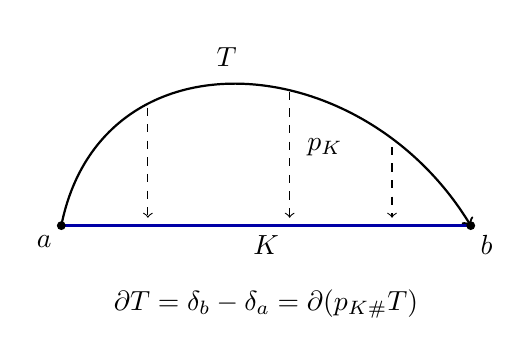
\begin{tikzpicture}[x=1cm,y=1cm]
	\draw[very thick,blue!65!black] (-2.6,0)--(2.6,0);
	\node[below] at (0,0) {\(K\)};
	\draw[thick,->] (-2.6,0) .. controls (-2.1,2.5) and (1.2,2.3) .. (2.6,0);
	\node[above] at (-0.5,1.9) {\(T\)};
	\draw[dashed,->] (-1.5,1.5)--(-1.5,0.1);
	\draw[dashed,->] (0.3,1.7)--(0.3,0.1);
	\draw[dashed,->] (1.6,1)--(1.6,0.1);
	\node[right] at (0.4,1) {\(p_K\)};
	\fill (-2.6,0) circle (1.6pt) node[below left] {\(a\)};
	\fill (2.6,0) circle (1.6pt) node[below right] {\(b\)};
	\node at (0,-1) {\(\partial T=\delta_b-\delta_a=\partial(p_{K\#}T)\)};
\end{tikzpicture}

	\caption[把竞争者投影到紧凸集]{把竞争者投影到紧凸集。图中以线段 \(K\) 和弧线示意一维情形；端点保持不动，弧线的推前落在 \(K\) 上。一般维数使用同一个 \(1\)-Lipschitz 估计控制质量。}
	\label{g3:fig:plateau-convex-projection}
\end{figure}

\subsection{极小化序列及质量界}
\label{g3:subsec:2301:04}
设 \(B\) 可填充，选定上述 \(K\)，并取一个初始竞争者 \(T_0\)。由下确界定义，对每个正整数 \(j\) 可选 \(R_j\in\mathcal A(B)\)，使
\[
	m(B)\le\mathbf M(R_j)\le m(B)+j^{-1}.
\]
令 \(T_j=p_{K\#}R_j\)。前一命题给出
\begin{equation}\label{g3:eq:plateau-minimizing-sequence}
\begin{aligned}
	&\operatorname{spt}T_j\subset K,\qquad \partial T_j=B,\\
	&m(B)\le\mathbf M(T_j)\le m(B)+j^{-1}
	\le\mathbf M(T_0)+1,\\
	&\mathbf N(T_j)=\mathbf M(T_j)+\mathbf M(B)
	\le\mathbf M(T_0)+1+\mathbf M(B).
\end{aligned}
\end{equation}
于是第22章紧性定理的全部条件已经具备：流为整数，支集共同紧，质量与边界质量有统一上界。边界质量之所以没有另外的估计困难，是因为竞争类从一开始就固定了整个边界流，而不只是边界所在的点集。

\ProseParagraphBreak
这种局部化思路见\cite[第34节，引理34.1及证明，第196--197页]{Simon1983}。这里把有限总质量但可能非紧支的竞争者也纳入比较，并显式核对投影对边界和整数性的作用。下一节从这列流出发，逐步识别极限及其质量。
% 纲要条目排为编号小节标题，并进入目录与书签；说明段仍保留于纲要注释中。

% !TeX root = ../../Book3.tex
% 纲要标题：### 23.2 整数流 Plateau 问题的存在性
% 纲要位置：几何学计划纲要.md，第 3082 行。
% 正文状态：初稿；尚未正式审核。

% 纲要内容开始
% 
% * 极小化序列的整数流极限
% * 边界算子的连续性
% * 质量下半连续
% * 极小填充的存在性
% * 极限中的拓扑变化
% 
% 纲要内容结束

\section{整数流 Plateau 问题的存在性}
\label{g3:sec:2302}
现在已有一列共同支于紧凸集的整数流，其质量趋于 \(m(B)\)，边界始终为 \(B\)。紧性给出极限对象；要把它认作解，还须分别检查它留在竞争类中以及它的质量达到下确界。把这两项检查分开，也能看清直接法在其他变分问题中需要哪些条件。

\subsection{极小化序列的整数流极限}
\label{g3:subsec:2302:01}
\begin{proposition}\label{g3:prop:plateau-limit-integer}
	设 \(1\le k\le n\)，\(B\in\mathcal I_{k-1}(\mathbb R^n)\) 紧支且可填充，\(K\) 为包含 \(\operatorname{spt}B\) 的非空紧凸集。由式\eqref{g3:eq:plateau-minimizing-sequence}选取的极小化序列有子列及 \(T_*\in\mathcal I_k(\mathbb R^n)\)，满足
	\[
		\operatorname{spt}T_*\subset K,\qquad
		\mathcal F(T_j-T_*)\longrightarrow0,
		\qquad T_j\rightharpoonup T_*.
	\]
\end{proposition}
\begin{proof}
	式\eqref{g3:eq:plateau-minimizing-sequence}给出共同紧支及
	\(\sup_j[\mathbf M(T_j)+\mathbf M(\partial T_j)]<\infty\)。逐项满足\cref{g3:thm:federer-fleming-compactness}的条件，所以有整数流子列极限及所述收敛。支集也可直接检查：若测试形式支于 \(\mathbb R^n\setminus K\)，每个 \(T_j\) 在其上均为零，故极限也为零。
\end{proof}

这里的整数性来自第22章已经证明的闭包定理。只对流的系数测度使用弱紧性，首先得到的是正规流；该步骤本身不会恢复可整流承载集和整数重数。前章关于切片的论证正好补齐了这部分。

\subsection{边界算子的连续性}
\label{g3:subsec:2302:02}
对任意 \(\eta\in\mathcal D^{k-1}(\mathbb R^n)\)，定义边界的公式给出
\begin{equation}\label{g3:eq:plateau-limit-boundary}
	\partial T_*(\eta)=T_*(\mathrm d\eta)
	=\lim_jT_j(\mathrm d\eta)
	=\lim_j\partial T_j(\eta)=B(\eta).
\end{equation}
因此 \(\partial T_*=B\)，极限确实属于 \(\mathcal A_K(B)\)。证明只用了 \(\mathrm d\eta\) 仍是紧支光滑测试形式，未要求边界在点集意义下逐点收敛。

\ProseParagraphBreak
例如，一列很薄的矩形边界可作为流趋于零，其支集却趋向一条非空线段。故“流的边界为 \(B\)”是一个有向积分恒等式，不能用“承载集的拓扑边界等于 \(\operatorname{spt}B\)”替换。整数流表示中的公共边可以因取向相反而抵消，重数也参与边界计算。

\subsection{质量下半连续}
\label{g3:subsec:2302:03}
若 \(\omega\) 为余质量至多一的紧支光滑 \(k\) 形式，则
\[
	T_*(\omega)=\lim_jT_j(\omega)\le\liminf_j\mathbf M(T_j).
\]
对 \(\omega\) 取上确界，即得\cref{g3:prop:current-mass-lsc}在此处的结论
\begin{equation}\label{g3:eq:plateau-limit-lsc}
	\mathbf M(T_*)\le\liminf_j\mathbf M(T_j)=m(B).
\end{equation}
另一方面，\(T_*\in\mathcal A(B)\) 使 \(m(B)\le\mathbf M(T_*)\)。两个方向合并后才得到质量相等。下半连续本身容许抵消损失，而极小化序列的极限仍属同一竞争类，使这种损失不能把质量降到下确界以下。

\begin{proposition}\label{g3:prop:plateau-minimizing-mass-measures}
	在上述极小化序列及其收敛子列下，有
	\[
		\mathbf M(T_j)\longrightarrow\mathbf M(T_*),\qquad
		\|T_j\|\rightharpoonup\|T_*\|
	\]
	作为支于 \(K\) 的有限 Radon 测度收敛。后一项指对每个连续函数的积分收敛，不表示 \(\mathbf M(T_j-T_*)\to0\)。
\end{proposition}
\begin{proof}
	总质量收敛已由下确界的两侧不等式得到。质量测度支于紧集 \(K\)，总量有界，所以任取子列都可再取弱收敛子列，记其极限为 \(\lambda\)。加权下半连续性说明，对每个非负紧支连续函数 \(\varphi\)，
	\[
		\int\varphi\,\mathrm d\|T_*\|\le\int\varphi\,\mathrm d\lambda.
	\]
	故 \(\lambda-\|T_*\|\) 是非负测度。取在 \(K\) 上等于一的 \(\varphi\)，总质量收敛又说明这个差测度的总量为零。因此 \(\lambda=\|T_*\|\)。任意子列的测度极限均相同，就得到整条已选流子列上的质量测度收敛。
\end{proof}

\subsection{极小填充的存在性}
\label{g3:subsec:2302:04}
\begin{theorem}[欧氏整数流 Plateau 存在性]\label{g3:thm:euclidean-plateau-existence}
	设 \(1\le k\le n\)，\(B\in\mathcal I_{k-1}(\mathbb R^n)\) 紧支，且存在有限质量整数流 \(T_0\in\mathcal I_k(\mathbb R^n)\) 满足 \(\partial T_0=B\)。则存在紧支整数流 \(T_*\in\mathcal I_k(\mathbb R^n)\)，使
	\begin{equation}\label{g3:eq:plateau-global-minimum}
		\partial T_*=B,\qquad
		\mathbf M(T_*)=\inf\{\mathbf M(S):
		S\in\mathcal I_k(\mathbb R^n),\ \partial S=B\}.
	\end{equation}
	若 \(B\ne0\)，可以取 \(\operatorname{spt}T_*\subset
	\overline{\operatorname{conv}}(\operatorname{spt}B)\)。若 \(B=0\)，唯一的质量极小者为零流。
\end{theorem}
\begin{proof}
	当 \(B=0\) 时，零流可容许，质量非负且质量为零当且仅当流为零，结论成立。以下设 \(B\ne0\)，取其支集的闭凸包为 \(K\)。它是非空紧凸集。

	初始竞争者使 \(0\le m(B)\le\mathbf M(T_0)<\infty\)。\cref{g3:prop:plateau-convex-reduction}将所有有限质量竞争者投影到 \(K\)，并证明受限前后的下确界相同。由式\eqref{g3:eq:plateau-minimizing-sequence}选择受限极小化序列，\cref{g3:prop:plateau-limit-integer}给出支于 \(K\) 的整数流极限 \(T_*\)。式\eqref{g3:eq:plateau-limit-boundary}保证 \(\partial T_*=B\)，式\eqref{g3:eq:plateau-limit-lsc}保证 \(\mathbf M(T_*)\le m(B)\)。最后用 \(T_*\) 本身的可容许性得到反向不等式，故 \(\mathbf M(T_*)=m(B)\)。下确界针对的是全部 \(\mathcal A(B)\)，所以极小性不限于支于 \(K\) 的竞争者。
\end{proof}

如果将 \(T_*\) 在一个有界开集内作紧支整数闭流扰动 \(Z\)，则 \(\partial(T_*+Z)=B\)，从而质量不会减小。更局部地，若 \(\operatorname{spt}Z\Subset W\)，在 \(W\) 外两流一致，减去相同的外部质量便有
\[
	\|T_*\|(W)\le\|T_*+Z\|(W).
\]
这就是后面内部正则性所需的局部绝对面积极小性质。定理没有给出一般的唯一性；证明中选取子列也允许不同极小化序列产生不同解。

\ProseParagraphBreak
为了计算一个确切最小值，把第19章的校准比较延伸到当前竞争类。那里“余范数”与第22章测试形式的“余质量”表示同一个 comass 范数。闭形式保持有向积分，余质量界将该积分与质量比较。

\begin{proposition}\label{g3:prop:euclidean-current-calibration}
	设 \(1\le k\le n\)，\(\phi\) 为 \(\mathbb R^n\) 上光滑闭 \(k\) 形式，处处满足 \(\|\phi_x\|_*\le1\)。若有限质量整数流
	\(T=\lBrack E,\tau,\theta\rBrack\)，其中 \(\theta>0\)，满足
	\(\langle\phi(x),\tau(x)\rangle=1\) 在 \(\|T\|\)-几乎处处成立，则对每个有限质量整数流 \(S\) 且 \(\partial S=\partial T\)，有 \(\mathbf M(T)\le\mathbf M(S)\)。
\end{proposition}
\begin{proof}
	有限质量流可以通过向量测度表示作用于有界光滑形式，所以 \(T(\phi)\)、\(S(\phi)\) 均有意义。先证明两者相等，并处理可能的非紧支集。

	径向同伦给出一个全局原始形式
	\[
		\alpha_x(v_1,\ldots,v_{k-1})
		=\int_0^1t^{k-1}\phi_{tx}(x,v_1,\ldots,v_{k-1})\,\mathrm dt,
		\qquad \mathrm d\alpha=\phi.
	\]
	最后一个等式由对拉回形式沿 \(x\mapsto tx\) 求导并在 \(t\in[0,1]\) 积分得到；正次数形式在常值映射下的拉回为零，闭性消去了含 \(\mathrm d\phi\) 的项。这也可逐个坐标系数使用乘积法则验证。余质量界给出 \(\|\alpha_x\|_*\le |x|/k\)。

	令 \(Q=S-T\)，则 \(\partial Q=0\)。取前节所用 \(\chi_R\)，边界恒等式给出
	\[
		0=Q(\mathrm d(\chi_R\alpha))
		=Q(\chi_R\phi)+Q(\mathrm d\chi_R\wedge\alpha).
	\]
	第二项的绝对值不超过
	\(C_{n,k}\|Q\|(B_{2R}\setminus B_R)\)，因为该环域上 \(|\mathrm d\chi_R|\le C/R\)、\(\|\alpha\|_*\le2R/k\)。有限总质量使这个上界趋于零。第一项由控制收敛趋于 \(Q(\phi)\)，故 \(S(\phi)=T(\phi)\)。于是
	\[
		\mathbf M(T)=T(\phi)=S(\phi)\le\mathbf M(S).
	\]
	这证明了对全体有限质量竞争者的比较。
\end{proof}

在\cref{g3:exm:plateau-disk-initial}中，取常系数形式
\(\phi=\mathrm dx_1\wedge\mathrm dx_2\)，得到 \(m(B)=\pi R^2\)；边界为 \(qB\) 时，按 \(q\) 的正负选择 \(\phi\) 或 \(-\phi\)，得到 \(m(qB)=|q|\pi R^2\)。同样，对于两个不同点 \(a,b\)，常系数一形式
\(\phi=\langle(b-a)/|b-a|,\mathrm dx\rangle\) 校准从 \(a\) 到 \(b\) 的线段，故
\[
	m(\delta_b-\delta_a)=|b-a|.
\]
这些下界比较的是所有整数流竞争者，而不是只比较光滑图形。

\subsection{极限中的拓扑变化}
\label{g3:subsec:2302:05}
取 \(\mathbb R^3\) 中的单位圆盘 \(D\)，并在它上方放置半径 \(\varepsilon\) 的球面 \(S_\varepsilon\)，球心为 \((0,0,3\varepsilon)\)。两个承载集不相交。按各自取向令
\[
	T_\varepsilon=\lBrack D\rBrack+\lBrack S_\varepsilon\rBrack.
\]
则
\[
	\partial T_\varepsilon=\partial\lBrack D\rBrack,\qquad
	\mathbf M(T_\varepsilon)=\pi+4\pi\varepsilon^2\longrightarrow\pi,
\]
且球体填充给出
\(\mathcal F(T_\varepsilon-\lBrack D\rBrack)\le4\pi\varepsilon^3/3\)。这是一列极小化序列，其闭球面分支在极限中消失。固定边界并没有固定分支数。

\ProseParagraphBreak
即使要求曲面连通，细把手也可消失。具体地，在一个固定平面圆片内部去掉两个小圆盘，用上半空间中一条弧线的细管把两个圆周连接，再在接缝处光滑倒圆，得到与原圆片在外缘邻域一致的嵌入定向曲面。弧线可取半圆，管半径取为其半径的十分之一；管壁与外侧平面之间的两个直角接缝用固定光滑截面连接。这样得到一个具有有限面积的固定模型，外缘不动，内部增加一个把手。

\ProseParagraphBreak
把该模型按比例 \(\varepsilon\) 缩小，替换 \(D\) 内部半径 \(C\varepsilon\) 的圆片，记所得曲面为 \(D_\varepsilon\)。它仍连通，边界仍是单位圆，亏格增加一。修改只发生在直径 \(O(\varepsilon)\) 的区域，且新旧两片面积都为 \(O(\varepsilon^2)\)，故
\[
	\mathbf M(\lBrack D_\varepsilon\rBrack-\lBrack D\rBrack)
	\le C'\varepsilon^2,\qquad
	\mathbf M(\lBrack D_\varepsilon\rBrack)\longrightarrow\pi.
\]
所以固定亏格的光滑竞争者也可能收敛到不同亏格的流。Plateau 存在性保留的是定义中指定的整数结构与边界条件；拓扑约束是否保留，要在相应的更小竞争类中单独研究。

\ProseParagraphBreak
最后，质量相等也不会把平坦收敛加强为质量范数收敛。令 \(G_\varepsilon\) 为单位圆盘上函数 \(u_\varepsilon(x)=\varepsilon(1-|x|^2)\) 的向上定向图，则边界固定，面积趋于 \(\pi\)。图面在圆盘内部与 \(D\) 不交，而边界的一维集合没有二维质量，因此
\[
	\mathbf M(\lBrack G_\varepsilon\rBrack-\lBrack D\rBrack)
	=\mathbf M(\lBrack G_\varepsilon\rBrack)+\pi\longrightarrow2\pi.
\]
两者之间的竖向同伦却有质量 \(O(\varepsilon)\)，且侧边固定，故其平坦距离趋于零。这与\cref{g3:prop:plateau-minimizing-mass-measures}的质量测度弱收敛完全相容。
% 纲要条目排为编号小节标题，并进入目录与书签；说明段仍保留于纲要注释中。

% !TeX root = ../../Book3.tex
% 纲要标题：### 23.3 单调性、切锥与正则点
% 纲要位置：几何学计划纲要.md，第 3090 行。
% 正文状态：初稿；尚未正式审核。

% 纲要内容开始
% 
% * 第一变分和驻值
% * 密度及放大极限
% * 平面切锥与正则性问题
% * 极小整数流的内部与边界正则性
% 
% 纲要内容结束

\section{单调性、切锥与正则点}
\label{g3:sec:2303}
极小化给出一个整数流之后，还要辨认它在小尺度上的形状。可以先用光滑微分同胚移动这个流；极小性使质量的一阶变化为零，径向移动进而比较同一中心的不同尺度。缩小观察尺度得到切锥，它保留面积密度与重数。最后需要正则性定理，把足够平坦的弱对象恢复成光滑曲面。本节完整推导第一变分和单调性；极小流的质量收敛以及一般正则性采用下文逐项注明的外部结果。

\subsection{第一变分和驻值}
\label{g3:subsec:2303:01}
设 \(U\subset\mathbb R^n\) 开，\(1\le k<n\)。本节的局部质量极小，是指局部整数 \(k\) 流 \(T\) 满足：对每个 \(W\Subset U\) 及支于 \(W\) 内某个紧集的整数 \(k\) 流 \(Z\)，只要 \(\partial Z=0\)，就有
\[
	\|T\|(W)\le\|T+Z\|(W).
\]
由前节得到的全空间固定边界极小流满足这个条件。下面只在 \(U\cap\operatorname{spt}\partial T=\varnothing\) 的区域讨论内部变分。

\ProseParagraphBreak
将 \(T\) 写成 \(\lBrack E,\tau,\theta\rBrack\)，其中 \(\theta\) 取正整数，取向的符号吸收到 \(\tau\) 中。记 \(P_x\) 为 \(E\) 在几乎每点的近似切平面，\(\mu=\|T\|=\theta\mathcal H^k\llcorner E\)。对 \(C^1\) 向量场 \(X\)，定义沿 \(P_x\) 的散度
\[
	\operatorname{div}_{P_x}X
	=\sum_{i=1}^k\langle \mathrm DX(x)e_i,e_i\rangle,
\]
其中 \(e_1,\ldots,e_k\) 是 \(P_x\) 的任意正交单位基。它是 \(\mathrm DX\) 在该平面上的迹，因而不依赖基的选择。

\begin{theorem}\label{g3:thm:minimizing-current-stationarity}
	设 \(T\) 是开集 \(U\subset\mathbb R^n\) 中局部质量极小的整数 \(k\) 流，\(\partial T=0\) 于 \(U\)，\(1\le k<n\)。记 \(\mu=\|T\|\)，\(P_x\) 为其可整流表示的近似切平面，\(\operatorname{div}_{P_x}\) 为切向散度。则对每个 \(X\in C_c^1(U;\mathbb R^n)\)，都有
	\begin{equation}\label{g3:eq:current-stationarity}
		\delta T(X)\coloneqq\int\operatorname{div}_{P_x}X\,\mathrm d\mu(x)=0.
	\end{equation}
\end{theorem}
\begin{proof}
	先取光滑 \(X\)，令 \(\Phi_t\) 为它的小时间流。选 \(W\Subset U\)，使 \(X\) 的支集紧含于 \(W\)。\(\Phi_t\) 在 \(W\) 边界附近为恒等。第22章的推前与同伦公式说明 \(\Phi_{t\#}T-T\) 紧支于 \(W\)，其边界为零，故是允许的局部竞争变化。

	微分同胚单射，推前时没有不同原像之间的取向抵消。\cref{g3:prop:rectifiable-lipschitz-pushforward}的面积公式于是给出
	\[
		\|\Phi_{t\#}T\|(W)
		=\int_{E\cap W}J_k(\mathrm D\Phi_t|_{P_x})\,\theta\,\mathrm d\mathcal H^k.
	\]
	在 \(P_x\) 的正交基下，Jacobian 是 Gram 行列式的平方根。由
	\(\mathrm D\Phi_t=I+t\mathrm DX+o(t)\)，得到
	\[
		\left.\frac{\mathrm d}{\mathrm dt}\right|_{t=0}
		J_k(\mathrm D\Phi_t|_{P_x})
		=\sum_{i=1}^k\langle\mathrm DXe_i,e_i\rangle.
	\]
	余项在包含 \(\operatorname{spt}X\) 的紧集以及全部 \(k\) 平面上均匀；局部质量有限允许在积分号下求导。正负 \(t\) 都是竞争参数，极小性迫使导数为零，得到式\eqref{g3:eq:current-stationarity}。最后用同一紧支集上的光滑 \(C^1\) 逼近推广到 \(C_c^1\) 向量场。
\end{proof}

我们把满足式\eqref{g3:eq:current-stationarity}的可整流质量分布称为\term[zhuzhi]{驻值}[stationary]的。这个条件只使用 \(P_x\) 与正质量 \(\mu\)，不使用切平面的取向。若 \(E\) 是光滑无边界子流形，它恢复第19章的面积驻值公式：本书光滑平均曲率 \(H\) 是第二基本形式迹的 \(1/k\)，所以
\(\delta T(X)=-k\int\langle H,X\rangle\,\mathrm d\mu\)
在重数局部常值的区域成立。驻值是一阶条件；它不自动给出任意竞争流的质量比较。

\subsection{密度及放大极限}
\label{g3:subsec:2303:02}
取向消失于第一变分之后，径向计算与光滑情形具有同一形式。所需的是几乎处处的切平面，不需要先知道支集是一张光滑曲面。

\begin{theorem}\label{g3:thm:stationary-current-monotonicity}
	设 \(T\) 为 \(U\subset\mathbb R^n\) 中局部整数 \(k\) 流，\(1\le k<n\)，记 \(\mu=\|T\|\)、\(P_x\) 为近似切平面，并假定其质量分布满足式\eqref{g3:eq:current-stationarity}。若 \(\overline B_R(a)\subset U\)，则
	\[
		r\longmapsto\frac{\mu(B_r(a))}{r^k}
	\]
	在 \((0,R)\) 上单调不减。对满足
	\(\mu(\partial B_s(a))=\mu(\partial B_t(a))=0\)
	的 \(0<s<t<R\)，有精确差值式
	\begin{equation}\label{g3:eq:current-monotonicity-difference}
		\frac{\mu(B_t(a))}{t^k}-\frac{\mu(B_s(a))}{s^k}
		=\int_{B_t(a)\setminus B_s(a)}
		\frac{|(x-a)^{\perp P_x}|^2}{|x-a|^{k+2}}\,\mathrm d\mu(x).
	\end{equation}
\end{theorem}
\begin{proof}
	平移后取 \(a=0\)。令 \(r=|x|\)，先在径向光滑截断
	\(X(x)=\gamma(r)x\) 中计算。因为
	\(\sum_i\langle x,e_i\rangle^2=|x^{P_x}|^2\)，有
	\[
		\operatorname{div}_{P_x}X
		=k\gamma(r)+r\gamma'(r)
		-\frac{\gamma'(r)}r|x^{\perp P_x}|^2.
	\]
	选择如下连续、分段光滑的截断：
	\[
		\gamma(r)=
		\begin{cases}
			s^{-k}-t^{-k},&0\le r\le s,\\
			r^{-k}-t^{-k},&s<r<t,\\
			0,&r\ge t.
		\end{cases}
	\]
	它在原点附近为常数。只在 \(s,t\) 附近作光滑化，函数及其导数保持一致有界；由于两个球面的 \(\mu\) 质量为零，可用控制收敛将它代入驻值等式。\(r<s\) 的散度是 \(k(s^{-k}-t^{-k})\)；\(s<r<t\) 上的散度是
	\(-kt^{-k}+k|x^{\perp P_x}|^2r^{-k-2}\)。积分相加，再除以 \(k\)，便得到式\eqref{g3:eq:current-monotonicity-difference}。

	右侧非负，故质量比在这些良好半径之间单调。坏半径至多可数，因为不同球面互不相交，而 \(\mu\) 在 \(B_R(a)\) 内有限。对任意 \(s<t\)，分别取良好半径从下方趋于 \(s,t\)；开球递增并覆盖目标开球，测度的下连续性遂把单调性推广到全部半径。
\end{proof}

\begin{corollary}\label{g3:cor:minimizing-current-density}
	设 \(U\subset\mathbb R^n\) 开，\(1\le k<n\)，\(T\) 为 \(U\) 中局部整数 \(k\) 维流，\(\mu=\|T\|\)，且 \(\int\operatorname{div}_{P_x}X\,\mathrm d\mu=0\) 对所有 \(X\in C_c^1(U;\mathbb R^n)\) 成立；这里 \(P_x\) 为近似切平面，\(\theta\) 为整数重数。则每个 \(a\in U\) 都存在有限密度
	\[
		\Theta^k(\mu,a)
		=\lim_{r\downarrow0}\frac{\mu(B_r(a))}{\omega_kr^k}.
	\]
	在 \(\mu\)-几乎每点，此密度等于整数重数 \(\theta(a)\)。若 \(a\in\operatorname{spt}T\)，则 \(\Theta^k(\mu,a)\ge1\)。特别地，在球不遇 \(U\) 边界时，
	\begin{equation}\label{g3:eq:stationary-integer-mass-lower-bound}
		\mu(B_r(a))\ge\omega_kr^k.
	\end{equation}
\end{corollary}
\begin{proof}
	单调性使质量比在趋零时有极限，其值不超过任意固定内球的有限质量比。\cref{g3:thm:weighted-rectifiable-density}适用于整数重数表示：\(\theta\ge1\) 使载体在局部具有有限 \(\mathcal H^k\) 测度，所以几乎处处的密度是 \(\theta\)。

	这些密度至少为一的点在支集中稠密。给定 \(a\in\operatorname{spt}T\)，取这样的点 \(a_j\to a\)。对固定 \(r\) 及充分大的 \(j\)，球
	\(B_{r-|a_j-a|}(a_j)\) 包含于 \(B_r(a)\)。在 \(a_j\) 处使用单调性和密度下界，再令 \(j\to\infty\)，得到式\eqref{g3:eq:stationary-integer-mass-lower-bound}。最后令 \(r\downarrow0\)。
\end{proof}

现在固定内部点 \(a\in\operatorname{spt}T\)，用
\[
	\eta_{a,r}(x)=\frac{x-a}{r},\qquad T_{a,r}=\eta_{a,r\#}T
\]
放大。推前本身已含 \(k\) 阶 Jacobian，质量满足
\(\|T_{a,r}\|(B_R)=r^{-k}\mu(B_{Rr}(a))\)，不再另乘 \(r^{-k}\)。对每个固定 \(R\)，单调性给出这些质量的一致上界，而充分小的 \(r\) 使放大流在 \(B_R\) 中无边界。\cref{g3:thm:local-integral-current-compactness}因此给出局部整数弱极限。

\ProseParagraphBreak
要把它称作切锥，还需要防止质量在弱极限中抵消。这里调用极小流特有的紧性加强，其证明通过切片粘合小误差，使极限的竞争者能转移回原序列。精确外部输入如下；来源是\cite[定理34.5及注34.6(1)，第198--202页]{Simon1983}。

\begin{theorem}\label{g3:thm:minimizing-current-mass-compactness}
	设 \(U\subset\mathbb R^n\) 开，\(T_j\) 为 \(U\) 中局部质量极小的整数 \(k\) 流，\(\partial T_j=0\) 于 \(U\)。若它们在每个 \(W\Subset U\) 上质量一致有界，并且 \(T_j\rightharpoonup T\)，则 \(T\) 仍局部质量极小且为整数流，并有
	\[
		\|T_j\|\rightharpoonup\|T\|
	\]
	作为局部 Radon 测度收敛。
\end{theorem}

上述定理在此作为外部结果使用。它比第22章的整数流紧性多给出质量测度收敛与极小性的保持；单独的下半连续性没有这些结论。位置与切平面的联合测度将在\secref{g3:sec:2304}中正式定义为变分流形。

\begin{theorem}\label{g3:thm:minimizing-current-tangent-cone}
	设 \(T\) 是 \(U\subset\mathbb R^n\) 中局部质量极小的整数 \(k\) 流，\(\partial T=0\) 于 \(U\)，\(1\le k<n\)。记 \(T_{a,r}=(x\mapsto(x-a)/r)_\#T\)。给定 \(a\in\operatorname{spt}T\) 和任意 \(r_j\downarrow0\)，可取子列使 \(T_{a,r_j}\rightharpoonup C\) 局部收敛，其中 \(C\ne0\) 是 \(\mathbb R^n\) 中局部质量极小、无边界的整数流，满足
	\begin{equation}\label{g3:eq:current-tangent-cone-homogeneity}
		D_{\lambda\#}C=C\quad(\lambda>0),\qquad D_\lambda(x)=\lambda x,
	\end{equation}
	以及
	\[
		\|C\|(B_R)=\omega_kR^k\Theta^k(\|T\|,a)\quad(R>0).
	\]
	这样的 \(C\) 称为 \(T\) 在 \(a\) 的\term[qiezhui]{切锥}[tangent cone]。
\end{theorem}
\begin{proof}
	前述局部质量界与整数紧性先给出 \(C\)。每个放大流仍在相应放大开集内质量极小；对任意固定球，充分大的 \(j\) 都满足外部定理的假设。逐球使用\cref{g3:thm:minimizing-current-mass-compactness}，知 \(C\) 极小，且质量测度局部收敛。

	当 \(\|C\|(\partial B_R)=0\) 时，测度收敛给出
	\[
		\|C\|(B_R)
		=\lim_jr_j^{-k}\mu(B_{Rr_j}(a))
		=\omega_kR^k\Theta^k(\mu,a).
	\]
	这样的半径除至多可数个外任意。由良好半径从两侧逼近，知这个等式对全部 \(R>0\) 成立，且所有球面均为 \(\|C\|\) 零测集。密度下界保证 \(C\ne0\)。

	\(C\) 是驻值的，且其质量比恒定。将差值式\eqref{g3:eq:current-monotonicity-difference}用于 \(C\)，得到
	\(x\in P_x\) 在 \(\|C\|\)-几乎处处成立。这还须转成流本身的齐次性。固定 \(\lambda>0\)，考虑
	\(F(t,x)=(1-t+t\lambda)x\)，\(0\le t\le1\)。时间方向的导数是 \((\lambda-1)x\)，已在切平面内，因此 \(F\) 作用于 \([0,1]\times C\) 的 \((k+1)\) 维切向 Jacobian 为零。推前流因而为零。又 \(\partial C=0\)，同伦公式给出
	\[
		D_{\lambda\#}C-C
		=\partial F_\#([0,1]\times C)=0.
	\]
	这里缩放因子始终处于两个正数之间；对任意紧支测试形式，其逆像支集仍有界，故第22章的局部同伦公式适用。齐次性得证。
\end{proof}

这个结论保证每个放大序列都有切锥子列，未指定不同子列必有同一极限。切锥保留中心密度，却可能比原流的局部几何简单得多；下一小节的分支曲线正体现这一点。

\subsection{平面切锥与正则性问题}
\label{g3:subsec:2303:03}
称内部点 \(a\in\operatorname{spt}T\) 为正则点，是指某个邻域内
\(T=q\lBrack M\rBrack\)，其中 \(M\) 是光滑嵌入、无边界、定向的 \(k\) 维子流形，\(q\) 为正整数。其余内部支集点组成奇异集 \(\operatorname{Sing}_{\mathrm{int}}T\)。正则性描述支集和重数的局部表示，单独出现一张平面作为切锥还没有提供这种表示。

\ProseParagraphBreak
重数为一时，Allard\footnote{William Kenneth Allard（1941—），在美国工作的数学家，研究几何测度论，建立了变分流形的第一变分与正则性理论。}正则性给出明确结论。下面是其驻值整数流特例，作为外部正则性结果引用\cite[定理24.2，第125--128页；定理36.3，第211--212页]{Simon1983}；含 \(L^p\) 平均曲率的定量输入见\cref{g3:thm:allard-regularity}。

\begin{theorem}\label{g3:thm:unit-density-minimizing-current-regularity}
	设 \(T\) 是开集 \(U\subset\mathbb R^n\) 中局部质量极小、无边界的整数 \(k\) 流。若 \(a\in\operatorname{spt}T\) 满足
	\(\Theta^k(\|T\|,a)=1\)，则 \(a\) 是重数为一的正则点。特别地，若某个切锥是重数为一的定向平面流，则 \(a\) 正则。
\end{theorem}

说明调用条件如何出现：整数重数使几乎处处密度至少为一，驻值性使广义平均曲率为零，而中心密度为一使充分小球上的质量比任意接近一。Allard 定理把这三个条件变成一张 \(C^{1,\alpha}\) 单图；把流沿图投影推到参数平面，无边界条件与\cref{g3:thm:current-constancy}使所得顶维流的整数重数为常数；再沿图嵌入推回，并用中心密度为一确定该常数。在 Euclid 极小图方程下，局部椭圆正则性将它提升为光滑图。若从平面切锥出发，则上一小节的质量测度收敛先保证中心密度确为一。这个质量信息是把弱放大极限用于正则性判断的关键。

\begin{example}\label{g3:exm:complex-cusp-current}
	在 \(\mathbb C^2\cong\mathbb R^4\) 中取
	\[
		F(z)=(z^2,z^3),\qquad T=F_\#\lBrack\overline D\rBrack,
	\]
	其中 \(D\subset\mathbb C\) 为单位圆盘，取复定向。\(F\) 光滑，在 \(z\ne0\) 时是单射浸入：若 \(z^2=w^2\) 且 \(z^3=w^3\)，则 \(z=w\)。故 \(T\) 在原点之外的有效重数为一，边界是光滑嵌入曲线 \(F(\partial D)\)。

	标准二形式
	\(\omega=\mathrm dx_1\wedge\mathrm dy_1+\mathrm dx_2\wedge\mathrm dy_2\)
	由\cref{g3:prop:wirtinger-calibration}具有余质量一，并在每个正向复直线上取等。\(F\) 的非退化切平面均为复直线，故 \(T(\omega)=\mathbf M(T)\)。这个形式全局光滑、有界且闭，因此\cref{g3:prop:euclidean-current-calibration}适用，说明 \(T\) 在全部有限质量、同整数边界的竞争者中质量最小，特别地局部质量极小。

	令 \(b>0\) 满足 \(r^2=b^4+b^6\)。因为
	\(J_2F(z)=4|z|^2+9|z|^4\)，对充分小的 \(r\) 有
	\[
		\|T\|(B_r(0))
		=\int_{|z|<b}(4|z|^2+9|z|^4)\,\mathrm d\mathcal L^2(z)
		=2\pi b^4+3\pi b^6.
	\]
	所以 \(\Theta^2(\|T\|,0)=2\)。将参数改写为 \(z=\sqrt r\,w\)，放大后的参数化为
	\[
		w\longmapsto(w^2,\sqrt r\,w^3).
	\]
	任意固定紧支测试形式的原像位于一致有界的 \(w\) 域；参数化在该域光滑收敛到 \(w\mapsto(w^2,0)\)。于是全部放大流都趋于 \(2\lBrack\mathbb C\times\{0\}\rBrack\)，它是唯一的平面切锥。

	然而原点不是正则点。若支集在原点附近是 \(C^1\) 嵌入曲面，其切平面必为 \(\mathbb C\times\{0\}\)，到第一复坐标的投影将由逆函数定理局部单射。但 \(F(z)\) 与 \(F(-z)\) 在 \(z\ne0\) 时是不同点，却有相同的第一坐标 \(z^2\)，矛盾。这个例子同时具有质量极小性、光滑边界和唯一平面切锥，仍在内部出现分支奇点。
\end{example}

\subsection{极小整数流的内部与边界正则性}
\label{g3:subsec:2303:04}
密度一正则性处理最接近平面的单层情形。一般内部奇异集的大小还取决于维数与余维，尤其不能把超曲面的维数阈值用于高余维流。以下两项是本节采用的外部内部正则性结论。

\begin{theorem}\label{g3:thm:area-minimizing-interior-singular-bounds}
	设 \(U\subset\mathbb R^n\) 开，\(2\le k<n\)，\(T\) 为 \(U\) 中局部质量极小的整数 \(k\) 流，\(\partial T=0\) 于 \(U\)。
	\begin{enumerate}
		\item 在任意余维中，\(\operatorname{Sing}_{\mathrm{int}}T\) 的 Hausdorff 维数至多为 \(k-2\)，即对每个 \(\varepsilon>0\)，
		\[
			\mathcal H^{k-2+\varepsilon}(\operatorname{Sing}_{\mathrm{int}}T)=0.
		\]
		\item 若 \(n=k+1\)，则 \(k\le6\) 时内部无奇点；\(k=7\) 时内部奇异集局部有限；\(k\ge8\) 时其 Hausdorff 维数至多为 \(k-7\)。
	\end{enumerate}
\end{theorem}

第一项是 Almgren\footnote{Frederick Justin Almgren Jr.（1933--1997），美国数学家，主要研究几何测度论。}的一般内部正则性定理，此处采用\cite[第36节，第210--211页]{Simon1983}所陈述的 Euclid 特例，证明依赖多值函数及分支分析。第二项见\cite[第37节，尤其定理37.7及其证明，第215--223页]{Simon1983}；书中先证明局部有限周长集合边界的版本，再通过余维一极小整数流的局部分层分解处理整数重数。高重数分层的最大值原理以及维数降低是这项结论的组成部分，不能只把一般流直接认作一个集合的边界。

\ProseParagraphBreak
这里 \(k\) 是流的维数。例如二维整数流在 \(\mathbb R^3\) 中内部光滑；在 \(\mathbb R^4\) 中，一般结论只把内部奇异集的 Hausdorff 维数压到零，\cref{g3:exm:complex-cusp-current}确实出现一个奇点。维数为零本身不意味着集合局部有限，后一个更强断言需要另行给出对应定理。

\ProseParagraphBreak
边界正则性另有假设。我们选用如下余维一版本，外引 Hardt--Simon\footnote{Robert M. Hardt，在美国工作的数学家，研究几何测度论与偏微分方程。Leon Melvyn Simon（1945—），澳大利亚出生的数学家，研究极小曲面、几何测度论与偏微分方程。}的边界正则性定理；正式公告明确陈述于\cite[定理2，第263--264页]{HardtSimon1979BoundaryAnnouncement}。

\begin{theorem}\label{g3:thm:hardt-simon-boundary-regularity}
	设 \(U\subset\mathbb R^{k+1}\) 开，\(k\ge2\)，\(T\) 是 \(U\) 中局部绝对质量极小的整数 \(k\) 流。设在 \(U\) 中
	\[
		\partial T=\lBrack\Gamma\rBrack,
	\]
	其中 \(\Gamma\) 为无边界、定向、嵌入的 \(C^2\) \((k-1)\) 维子流形，系数为一。则存在 \(\Gamma\) 的开邻域 \(V\subset U\)，使 \(V\cap\operatorname{spt}T\) 局部为嵌入的 \(C^{1,\alpha}\) 超曲面，对每个 \(0<\alpha<1\) 成立。支集可在 \(\Gamma\) 处终止，也可穿过 \(\Gamma\)；在后一种情形，\(\Gamma\) 两侧的整数重数跳跃一。若 \(\Gamma\) 光滑，则边界处的表示也光滑。
\end{theorem}

本定理的绝对质量极小，仍按本节开始的紧支整数闭流竞争定义，而非只对光滑微分同胚驻值。它的边界是重数一的嵌入子流形，环境余维为一。穿越情形可从两个同向同心平面圆周看出：相应平面填充在内圆盘上重数为二、外环带上重数为一，内圆是流的边界所在，但支集在那里是一整张平面。因此“边界正则”不要求支集的拓扑边界处处等于 \(\operatorname{spt}\partial T\)。

\ProseParagraphBreak
高余维的边界即使局部光滑，也可能遇到其他极小片。例如在 \(\mathbb C^2\) 中，把第一复坐标平面上的半圆盘流与第二复坐标平面上的整圆盘流相加，并在原点附近观察。边界在那里只是一条光滑直线，两个复片都由同一个 \(\omega\) 校准，故和流局部质量极小；原点附近支集却是相交的两片，不能表示成一张嵌入带边界曲面。此例说明余维一边界定理的环境条件有实际作用。对于给定 Plateau 解，内部结论应在远离边界处使用，边界结论则逐点核查所选定理的边界重数、嵌入性与环境条件。
% 纲要条目排为编号小节标题，并进入目录与书签；说明段仍保留于纲要注释中。

% !TeX root = ../../Book3.tex
% 纲要标题：### 23.4* 变分流形与第一变分
% 纲要位置：几何学计划纲要.md，第 3097 行。
% 正文状态：初稿；尚未正式审核。

% 纲要内容开始
% 
% * Grassmann 丛上的测度
% * 一阶变分和广义平均曲率
% * 无取向极限及重数
% * 流与变分流形的边界及抵消
% * Allard 正则性定理
% 
% ---
% 
% 纲要内容结束

\OptionalSection{变分流形与第一变分}{g3:sec:2304}

取两张彼此靠近、取向相反的平面。它们作为流可以相消，面积却仍是两张平面的面积。如果研究的目标是面积的驻值及其极限，就需要保留位置、面积和切平面，而不让取向改变面积的符号。变分流形用 Grassmann 丛上的正测度实现这一点。这里先建立测度与变分的基本运算，再准确陈述把弱几何对象恢复为图像的 Allard 正则性定理。一般变分流形的定义和第一变分参见\cite[第38--39节，第227--235页]{Simon1983}；其中 Grassmann 丛上的弱收敛有别于该书第15节仅对权测度所用的收敛约定。

\subsection{Grassmann 丛上的测度}
\label{g3:subsec:2304:01}
设 \(U\subset\mathbb R^n\) 开，\(1\le k<n\)。记 \(G(n,k)\) 为 \(\mathbb R^n\) 中所有\emph{无取向}的 \(k\) 维线性子空间组成的 Grassmann 流形。把平面 \(P\) 与其正交投影矩阵 \(\pi_P\) 对应，则
\[
	G(n,k)=\{A\in\mathbb R^{n\times n}:A^{\mathsf T}=A,\ A^2=A,\ \operatorname{tr}A=k\}.
\]
这是矩阵空间中的闭有界集，因而紧。距离可取 \(|\pi_P-\pi_Q|\)。Euclid 情形的 Grassmann 丛是乘积
\[
	G_k(U)\coloneqq U\times G(n,k).
\]
其一点 \((x,P)\) 同时记录位置和经过该位置的平面方向；仿射切平面对应 \(x+P\)。

\begin{definition}\label{g3:def:varifold}
	设 \(U\subset\mathbb R^n\) 开，\(1\le k<n\)。记 \(G(n,k)\) 为 \(\mathbb R^n\) 的无取向 \(k\) 平面空间，\(G_k(U)=U\times G(n,k)\)。\(G_k(U)\) 上的非负 Radon 测度称为 \(U\) 中的 \(k\) 维\term[bianfen liuxing]{变分流形}[varifold]，记为 \(V\)。其\term[quanzhong cedu]{权测度}[weight measure]是位置投影 \(\pi(x,P)=x\) 的推前
	\[
		\mu_V(A)\coloneqq V(A\times G(n,k)),\qquad A\subset U\text{ 为 Borel 集}.
	\]
	权测度也记为 \(\|V\|\)。总质量为 \(\mu_V(U)\)，在环境中的支集指 \(\operatorname{spt}\mu_V\)。
\end{definition}
\symidx{\(\mu_V=\lVert V\rVert\)：变分流形的权测度}

Grassmann 纤维紧，故紧集 \(K\Subset U\) 的逆像 \(K\times G(n,k)\) 也紧，权测度在 \(U\) 上确为 Radon 测度。定义中的“变分”不表示已经满足某个极值条件；任意这样的非负测度都是变分流形。

\begin{definition}\label{g3:def:rectifiable-varifold}
	设 \(U\subset\mathbb R^n\) 开，\(1\le k<n\)，\(G_k(U)=U\times G(n,k)\) 为无取向切平面丛，\(M\subset U\) 是可数 \(k\)-可整流 Borel 集，\(\theta:M\to(0,\infty)\) 可测，并且 \(\int_{M\cap K}\theta\,\mathrm d\mathcal H^k<\infty\) 对每个 \(K\Subset U\) 成立。按 Lipschitz 片取几乎处处一致的切平面 \(\mathrm{T}_xM\)，以
	\begin{equation}\label{g3:eq:rectifiable-varifold}
		\mathbf v(M,\theta)(\varphi)
		=\int_M\varphi(x,\mathrm{T}_xM)\theta(x)\,\mathrm d\mathcal H^k(x),
		\qquad \varphi\in C_c(G_k(U)),
	\end{equation}
	定义的变分流形称为\term[kezhengliu bianfen liuxing]{可整流变分流形}[rectifiable varifold]。如果 \(\theta\) 几乎处处取正整数值，就称为\term[zheng bianfen liuxing]{整变分流形}[integral varifold]。重数为一时简记 \(\mathbf v(M)\)。
\end{definition}
\symidx{\(\mathbf v(M,\theta)\)：由可整流集及正重数定义的变分流形}

一般实重数可使整个承载集的局部 \(\mathcal H^k\) 测度无限；此时切平面按可数片确定，沿用\cref{g3:def:rectifiable-current}的约定。整数重数满足 \(\theta\ge1\)，于是有效承载集局部 \(\mathcal H^k\) 有限。式\eqref{g3:eq:rectifiable-varifold}给出
\[
	\mu_{\mathbf v(M,\theta)}=\theta\mathcal H^k\llcorner M.
\]
可整流流 \(T=\lBrack M,\tau,\theta\rBrack\) 所对应的变分流形记为
\begin{equation}\label{g3:eq:current-associated-varifold}
	V_T\coloneqq\mathbf v(M,|\theta|),\qquad \mu_{V_T}=\|T\|.
\end{equation}
这一构造忘掉 \(\tau\) 的正负，但保留其张成的平面。一个嵌入的 Möbius 带也直接给出 \(\mathbf v(M)\)，无需选择全局取向。

\begin{example}\label{g3:exm:diffuse-varifold}
	设 \(U\subset\mathbb R^n\) 为非空开集。取 \(1\le k<n\) 和两个不同平面 \(P,Q\in G(n,k)\)。测度
	\[
		V_P=\mathcal L^n\llcorner U\otimes\delta_P,\qquad
		V_Q=\mathcal L^n\llcorner U\otimes\delta_Q
	\]
	有相同权测度，却是不同的变分流形，因为可以用只依赖平面方向的连续函数区别它们。两者均非 \(k\) 维可整流：可数 \(k\)-可整流集的 \(n\) 维 Lebesgue 测度为零，无法承载 \(\mathcal L^n\llcorner U\)。所以权测度和维数标记本身不保证切向几何结构。
\end{example}

为比较变形前后的面积，推前还必须带上切向 Jacobian。设 \(f:U\to W\subset\mathbb R^q\) 为 \(C^1\) 映射，且在 \(\operatorname{spt}\mu_V\) 上对 \(W\) 固有。定义
\[
	J_Pf(x)=\sqrt{\det\bigl((\mathrm Df(x)|_P)^*\mathrm Df(x)|_P\bigr)}.
\]
这里假设 \(q\ge k\)。当此数非零时，\(\mathrm Df(x)P\) 是 \(k\) 维平面。令
\begin{equation}\label{g3:eq:varifold-pushforward}
	(f_\#V)(\varphi)=\int_{G_k(U)}
	\varphi(f(x),\mathrm Df(x)P)J_Pf(x)\,\mathrm dV(x,P),
\end{equation}
其中 \(J_Pf=0\) 的部分贡献定义为零。固有性及紧集上导数有界保证右侧对紧支连续测试函数有限，因此定义 Radon 测度。

\begin{proposition}\label{g3:prop:rectifiable-varifold-pushforward}
	设 \(V=\mathbf v(M,\theta)\) 是 \(U\subset\mathbb R^n\) 中可整流 \(k\) 维变分流形，\(f:U\to W\subset\mathbb R^q\) 为在 \(\operatorname{spt}\mu_V\) 上固有的 \(C^1\) 映射，\(q\ge k\)。则 \(f_\#V\) 可整流；若 \(V\) 整，则 \(f_\#V\) 也整。在满秩像点，其重数几乎处处为
	\[
		\theta_f(y)=\sum_{\substack{x\in M\cap f^{-1}(y)\\J_{\mathrm{T}_xM}f(x)>0}}\theta(x).
	\]
\end{proposition}
\begin{proof}
	局部把满秩参数域分成可数双 Lipschitz 片。其像为可整流片，重叠部分在几乎处处具有同一切平面。面积公式将式\eqref{g3:eq:varifold-pushforward}按像点重新积分，得到所示正重数之和；秩不足部分的像为 \(\mathcal H^k\) 零测集。每个紧集上的这个和可积，故在几乎每根纤维上有限。若各项为正整数，只有有限个非零项，和仍为整数。与流的推前相比，这里所有重数相加，不出现取向符号。
\end{proof}

\subsection{一阶变分和广义平均曲率}
\label{g3:subsec:2304:02}
令 \(X\in C_c^1(U;\mathbb R^n)\)，以 \(\Phi_t\) 表示它在小时间内生成的微分同胚。取紧集包含变形发生的区域，面积变化完全发生在这个紧集内；即使 \(V\) 总质量无限，也可以对这个局部质量差求导。定义
\[
	\operatorname{div}_P X(x)
	\coloneqq\operatorname{tr}(\pi_P\mathrm DX(x))
	=\sum_{i=1}^k\langle\mathrm D_{e_i}X,e_i\rangle,
\]
其中 \(e_1,\ldots,e_k\) 是 \(P\) 的任意正交单位基。迹的表示说明它与基无关。

\begin{proposition}\label{g3:prop:varifold-first-variation}
	设 \(V\) 为开集 \(U\subset\mathbb R^n\) 中 \(k\) 维变分流形。其沿 \(X\in C_c^1(U;\mathbb R^n)\) 的面积第一变分为
	\begin{equation}\label{g3:eq:varifold-first-variation}
		\delta V(X)=\int_{G_k(U)}\operatorname{div}_P X(x)\,\mathrm dV(x,P).
	\end{equation}
\symidx{\(\delta V\)：变分流形的第一变分}
	若右侧对所有这样的 \(X\) 为零，称 \(V\) 在 \(U\) 中驻值。
\end{proposition}
\begin{proof}
	固定 \(P\) 的一组正交单位基。\(\Phi_t\) 在 \(P\) 上的 Gram 矩阵为
	\[
		G_{ij}(t)=\langle\mathrm D\Phi_t e_i,\mathrm D\Phi_t e_j\rangle.
	\]
	在 \(t=0\)，\(G(0)=I\)，且
	\[
		G'_{ij}(0)=\langle\mathrm D_{e_i}X,e_j\rangle+
		\langle e_i,\mathrm D_{e_j}X\rangle.
	\]
	因此 \(\left.\frac{\mathrm d}{\mathrm dt}\right|_0J_P\Phi_t
	=\frac12\operatorname{tr}G'(0)=\operatorname{div}_PX\)。这个导数在变形的紧支集及紧 Grassmann 纤维上一致有界，故可以在式\eqref{g3:eq:varifold-pushforward}中求导。支集外 \(\Phi_t\) 为恒等，局部质量差的导数就是所示积分。
\end{proof}

第一变分目前由 \(X\) 的一阶导数控制。若对每个 \(K\Subset U\)，还存在常数 \(C_K\) 使
\[
	|\delta V(X)|\le C_K\|X\|_\infty
	\quad\text{当 }\operatorname{supp}X\subset K,
\]
就称 \(V\) 具有局部有界第一变分。分量上的 Riesz 表示给出唯一的向量 Radon 测度。相对于 \(\mu_V\) 作 Lebesgue 分解，可以唯一写成
\begin{equation}\label{g3:eq:varifold-mean-curvature-decomposition}
	\delta V(X)=-\int_U H_V\cdot X\,\mathrm d\mu_V+\int_U X\cdot\mathrm d\sigma_V,
	\qquad \sigma_V\perp\mu_V.
\end{equation}
\symidx{\(H_V,\sigma_V\)：变分流形的广义平均曲率与第一变分的奇异部分}
这里 \(H_V\in L^1_{\mathrm{loc}}(\mu_V;\mathbb R^n)\) 称为\term[guangyi pingjun qulv]{广义平均曲率}[generalized mean curvature]。\(\sigma_V\) 是第一变分的奇异部分，记录未被面积测度吸收的力项。将其称为广义边界力时，仍应记住它是环境中的向量测度。

\begin{proposition}\label{g3:prop:smooth-varifold-boundary-variation}
	设 \(M^k\subset U\subset\mathbb R^n\) 为在 \(U\) 中固有的 \(C^2\) 嵌入子流形，可带 \(C^2\) 边界，并且在每个紧集内 \(M\) 与 \(\partial M\) 的相应 Hausdorff 测度有限。对 \(V=\mathbf v(M)\) 及 \(X\in C_c^1(U;\mathbb R^n)\)，有
	\begin{equation}\label{g3:eq:smooth-varifold-variation}
		\delta V(X)=-k\int_M H\cdot X\,\mathrm d\mathcal H^k
		+\int_{\partial M}X\cdot\eta\,\mathrm d\mathcal H^{k-1},
	\end{equation}
	其中 \(H=k^{-1}\operatorname{tr}B\) 沿用\chapref{g3:ch:19}的平均曲率约定，\(\eta\) 为 \(M\) 内沿 \(\partial M\) 的外单位余法向。因此 \(H_V=kH\)、\(\sigma_V=\eta\mathcal H^{k-1}\llcorner\partial M\)。
\end{proposition}
\begin{proof}
	沿 \(M\) 分解 \(X=X^\top+X^\perp\)。由 \(\langle X^\perp,e_i\rangle=0\) 求导，
	\[
		\sum_i\langle\mathrm D_{e_i}X^\perp,e_i\rangle
		=-\sum_i\langle X^\perp,B(e_i,e_i)\rangle=-kH\cdot X.
	\]
	切向部分给出 \(\operatorname{div}_M X^\top\)。代入式\eqref{g3:eq:varifold-first-variation}，再对切向场应用子流形散度公式，得到边界通量 \(\int_{\partial M}X^\top\cdot\eta\)。因为 \(\eta\in\mathrm{T}M\)，这等于所示的 \(\int_{\partial M}X\cdot\eta\)。该散度公式也可在参数坐标中写成 \(\partial_i(\sqrt{\det g}\,X^i)\) 并用单位分解证明，因而不要求 \(M\) 可定向。边界的 \(k\) 维测度为零，故最后两项分别是相对于 \(\mu_V\) 的绝对连续部分与奇异部分。
\end{proof}

\begin{example}\label{g3:exm:varifold-sphere-and-segment}
	半径 \(R\) 的 \(k\) 维球面，沿外法向 \(\nu\) 有 \(H=-\nu/R\)，所以 \(H_V=-k\nu/R\)。取沿球面等于 \(x\) 的紧支向量场，式\eqref{g3:eq:smooth-varifold-variation}给出 \(\delta V(X)=k\mathcal H^k(S_R^k)>0\)，与放大时面积增加相符。

	对线段 \(M=\{te_1:a\le t\le b\}\)，内部曲率为零，而
	\[
		\delta\mathbf v(M)(X)=X(be_1)\cdot e_1-X(ae_1)\cdot e_1.
	\]
	第一变分全部集中于两端点。它的系数是余法向向量，与有向线段的零维边界流 \(\delta_{be_1}-\delta_{ae_1}\) 属于不同类型的对象。
\end{example}

对一般实重数变分流形，\(H_V\) 还可能有切向分量。若光滑正函数 \(\theta\) 赋予光滑 \(M\) 重数，积分分部给出
\[
	H_{\mathbf v(M,\theta)}=kH+\nabla_M\log\theta
\]
于无边界区域。这一切向项来自密度变化。下述 Allard 定理直接把 \(H_V\) 作为向量场控制，不预先删去它的切向部分。

\subsection{无取向极限及重数}
\label{g3:subsec:2304:03}
若 \(V_j,V\) 为 \(G_k(U)\) 上的变分流形，约定
\[
	V_j\rightharpoonup V
	\quad\Longleftrightarrow\quad
	V_j(\varphi)\longrightarrow V(\varphi)
	\quad\text{对每个 }\varphi\in C_c(G_k(U)).
\]
这同时测试位置和方向，立刻蕴含 \(\mu_{V_j}\rightharpoonup\mu_V\)。反向一般不成立，\cref{g3:exm:diffuse-varifold}已给出相同权测度可以对应不同方向分布的例子。

\begin{proposition}\label{g3:prop:varifold-weak-compactness}
	设 \(U\subset\mathbb R^n\) 开，\(V_j\) 为 \(k\) 维变分流形，并且对每个 \(K\Subset U\) 有 \(\sup_j\mu_{V_j}(K)<\infty\)。则存在子列弱收敛于某个 \(k\) 维变分流形 \(V\)。对每个固定 \(X\in C_c^1(U;\mathbb R^n)\)，
	\[
		\delta V_j(X)\longrightarrow\delta V(X).
	\]
	因此，若各 \(V_j\) 驻值，极限 \(V\) 也驻值。
\end{proposition}
\begin{proof}
	取 \(U\) 的可数紧耗尽及各 \(K\times G(n,k)\) 上连续函数的可数一致稠密族。局部质量界使每个测试积分有界，对这些积分逐次抽取子列并作对角选择。得到的极限泛函非负，且在各紧支集上由一致范数控制；Riesz 表示把它写成 Radon 测度 \(V\)。一致逼近再把收敛从可数稠密族扩展到所有紧支连续函数。

	函数 \((x,P)\mapsto\operatorname{div}_PX(x)\) 连续，支于 \(\operatorname{supp}X\times G(n,k)\)，故可直接作为弱收敛的测试函数。代入式\eqref{g3:eq:varifold-first-variation}即得第一变分的收敛和驻值性的保持。
\end{proof}

这条紧性只使用正测度和紧纤维，尚未恢复可整流性。下面的计算说明额外几何控制为什么有用。

\begin{example}\label{g3:exm:varifold-diffuse-limit}
	在单位方形 \(U=(0,1)^2\) 中，以 \(j\times j\) 方格的中心为中点，各放一条长度 \(j^{-2}\) 的水平线段，令 \(V_j\) 是这些线段的重数一变分流形之和。每条线段距其中心至多 \(1/(2j^2)\)，所以对 \(\varphi\in C_c(G_1(U))\)，一致连续性给出
	\[
		V_j(\varphi)-j^{-2}\sum_{a,b=0}^{j-1}
		\varphi\left(\left(\frac{a+1/2}{j},\frac{b+1/2}{j}\right),\mathbb Re_1\right)
		\longrightarrow0.
	\]
	右侧的 Riemann 和趋于 \(\int_U\varphi(x,\mathbb Re_1)\,\mathrm dx\)。因此各 \(V_j\) 都整、总质量都为一，极限却是弥散的 \(\mathcal L^2\llcorner U\otimes\delta_{\mathbb Re_1}\)。各线段端点的第一变分不能获得统一局部总变差界；它们在紧子方形中以 \(j^2\) 的量级增长。
\end{example}

\subsection{流与变分流形的边界及抵消}
\label{g3:subsec:2304:04}
流把取向写进测试形式的配对，变分流形把面积写成正测度。式\eqref{g3:eq:current-associated-varifold}在每个固定可整流流上连接两者，却不与加法、弱极限普遍相容。

\begin{example}\label{g3:exm:opposite-sheets-varifold-limit}
	在 \(\mathbb R^{k+1}=\mathbb R^k\times\mathbb R\) 中，令 \(P_t=\mathbb R^k\times\{t\}\)，各平面取相同的水平取向，考虑局部整数流
	\[
		T_j=\lBrack P_{1/j}\rBrack-\lBrack P_{-1/j}\rBrack.
	\]
	对任意紧支测试 \(k\) 形式，两个积分因平移趋于同一个值，故 \(T_j\rightharpoonup0\)。但对 \(\varphi\in C_c(G_k(\mathbb R^{k+1}))\)，
	\[
		V_{T_j}(\varphi)=\int_{\mathbb R^k}
		\bigl[\varphi((x,1/j),\mathbb R^k)+\varphi((x,-1/j),\mathbb R^k)\bigr]\,\mathrm dx
		\longrightarrow2\mathbf v(P_0)(\varphi).
	\]
	因此 \(V_{T_j}\rightharpoonup2\mathbf v(P_0)\ne V_0\)。这些变分流形及其极限都驻值，两张片的面积在极限中成为重数二。
\end{example}

在固定的共同可整流承载集上，加法时取向相反的系数可以抵消，故总有局部质量不等式
\[
	\|T_1+T_2\|\le\|T_1\|+\|T_2\|,
\]
而变分流形的非负测度直接相加。与之相应，整数流的条件 \(\partial T=S\) 指定了带系数和取向的边界；\(\delta V=0\) 则表示所有紧支环境变形的面积一阶导数为零。一个有边界的平坦圆盘在内部驻值，作为整个环境中的变分流形却有非零边界力。三个夹角均为 \(120^\circ\) 的射线则可以在公共端点平衡，形成整体驻值变分流形；它们的重数一有向链无法在公共端点使三个整数符号相加为零。

\ProseParagraphBreak
这解释了两个弱模型各自适合记录的数据。给定整数边界的 Plateau 问题使用 \(\partial T\) 的连续性；面积驻值极限和下面的几何极小极大构造使用正质量、切平面与 \(\delta V\) 的连续性。驻值条件只约束第一阶变化，不能替代同边界竞争类中的质量极小性。

\subsection{Allard 正则性定理}
\label{g3:subsec:2304:05}
一个对象在小球内的面积接近平面，仍可能带有多张片、弥散质量或边界力。\term[allard zhengzexing dingli]{Allard 正则性定理}[Allard regularity theorem]把这些问题放在可整流结构、密度下界和第一变分的准确条件中。以下采用\cite[第24节，假设24.1与定理24.2，第125--128页]{Simon1983}的球形版本，作为本节的外部正则性输入。

\begin{theorem}[Allard 正则性]\label{g3:thm:allard-regularity}
	设 \(1\le k<n\)、\(k<p<\infty\)，并令 \(\alpha=1-k/p\)。存在仅依赖 \(n,k,p\) 的常数 \(\varepsilon_0\in(0,1/2)\)、\(\gamma\in(0,1)\)、\(C<\infty\)，满足以下结论。设 \(V=\mathbf v(M,\theta)\) 是开集 \(U\subset\mathbb R^n\) 中的可整流 \(k\) 维变分流形，\(x_0\in\operatorname{spt}\mu_V\)、\(\overline B_R(x_0)\subset U\)，并且
	\begin{enumerate}
		\item \(\theta\ge1\) 在 \(B_R(x_0)\) 内 \(\mu_V\)-几乎处处成立；
		\item 在 \(B_R(x_0)\) 中，\(\delta V(X)=-\int H_V\cdot X\,\mathrm d\mu_V\)，其中 \(H_V\in L^p(\mu_V\llcorner B_R(x_0))\)，没有第一变分的奇异部分；
		\item 质量与曲率满足
		\[
			\frac{\mu_V(B_R(x_0))}{\omega_kR^k}\le1+\varepsilon_0,
			\qquad
			R^{1-k/p}\left(\int_{B_R(x_0)}|H_V|^p\,\mathrm d\mu_V\right)^{1/p}\le\varepsilon_0.
		\]
	\end{enumerate}
	则存在正交变换 \(Q\) 及函数 \(u\in C^{1,\alpha}(B_{\gamma R}^k(0);\mathbb R^{n-k})\)，使 \(u(0)=0\)，并且
	\[
		\operatorname{spt}\mu_V\cap B_{\gamma R}(x_0)
		=\bigl(x_0+Q(\operatorname{graph}u)\bigr)\cap B_{\gamma R}(x_0).
	\]
	它还满足尺度一致的估计
	\[
		R^{-1}\|u\|_\infty+\|\mathrm Du\|_\infty
		+R^\alpha[\mathrm Du]_{C^{0,\alpha}}
		\le C\varepsilon_0^{1/(4k)}.
	\]
\end{theorem}

这里的结论首先是\emph{支集}的单图表示；陈述允许实重数，因而不能由它把所有密度自动改成一。小质量比排除了重数二平面；\(\theta\ge1\) 排除了以很小权重叠加的额外薄片；\(\sigma_V=0\) 排除了圆盘边缘等内部边界力。指数 \(p>k\) 给出正 Hölder 指数，且使曲率项在缩小尺度时具有良好的衰减。若 \(|H_V|\le L\)，其尺度量至多为
\[
	R^{1-k/p}\|H_V\|_{L^p(B_R,\mu_V)}
	\le LR\left(\frac{\mu_V(B_R)}{R^k}\right)^{1/p}.
\]
这些条件都在所考察的球内检验，不能用球外的边界光滑性代替。

\begin{corollary}\label{g3:cor:multiplicity-one-varifold-regularity}
	设 \(V\) 是 \(U\subset\mathbb R^n\) 中驻值的整 \(k\) 维变分流形，\(1\le k<n\)，\(x\in\operatorname{spt}\mu_V\)。若存在 \(r_j\downarrow0\) 和 \(P\in G(n,k)\)，使
	\[
		(\eta_{x,r_j})_\#V\rightharpoonup\mathbf v(P),
		\qquad \eta_{x,r}(y)=\frac{y-x}{r},
	\]
	则对每个 \(0<\alpha<1\)，\(\operatorname{spt}\mu_V\) 在 \(x\) 的某个邻域内为一个 \(C^{1,\alpha}\) 图像。
\end{corollary}
\begin{proof}
	令 \(p=k/(1-\alpha)>k\)。Grassmann 测度收敛蕴含权测度收敛，而平面测度在 \(\partial B_1(0)\) 上为零，所以
	\[
		r_j^{-k}\mu_V(B_{r_j}(x))\longrightarrow\omega_k.
	\]
	整性给出重数下界一，驻值性给出 \(H_V=0\) 且 \(\sigma_V=0\)。当 \(j\) 充分大时，\(B_{r_j}(x)\Subset U\)，上式使 Allard 的小质量比成立。因此\cref{g3:thm:allard-regularity}在一个正半径的小球内给出所述图像。
\end{proof}

上述应用需要的是重数一的\emph{变分流形}放大极限。若最初只知道流的弱放大极限是一个平面，还须另外核对质量没有损失，才能得到这里的质量比。前节对极小流所用的质量收敛结论正承担这一步。一般驻值极限则可能保留较高重数，或出现射线交会这样的奇点。下一节的扫掠问题将利用驻值变分流形保存极小极大过程中留下的面积，并逐项说明何种额外理论保证整性、正则性与指标控制。

% !TeX root = ../../Book3.tex
% 纲要标题：### 23.5*　扫掠、宽度与极小极大方法
% 纲要位置：几何学计划纲要.md，第 3107 行。

% 纲要内容开始
% 
% > 写作范围与外部输入：规划任务：在第20—22章的弱极限工具与第23.4节变分流形之后引入几何 min-max。完整证明黎曼二球面上 Birkhoff 非平凡闭测地线的代表模块，交代离散缩短、宽度为正和极限不塌缩为常值；这不是第28章的平均曲率流。再在闭环境维数3—7及指定系数、扫掠空间和收敛拓扑下，准确外引所选 Almgren–Pitts 极小超曲面存在性，分别说明重数、正则性和指标。有限维山路模型只作动机，不替代几何存在证明；第16.4节谱的极小极大原则与本节另行辨析。
% 
% * 扫掠族、同伦约束与宽度
% * Birkhoff 曲线缩短
% * 二球面上的闭测地线
% * 超曲面扫掠与驻值变分流形
% * Almgren–Pitts 存在性定理
% * 维数、重数、正则性与指标的区别
% 
% ---
% 
% 纲要内容结束
% 正文状态：初稿；尚未正式审核。


\OptionalSection{扫掠、宽度与极小极大方法}{g3:sec:2305}
若把闭曲线的长度在所有闭曲线中直接取最小值，常值曲线已经给出零。要找到非恒定闭测地线，可以要求一整族曲线扫过球面，再降低这族曲线中最高的能量。单条曲线可以收缩，但整个扫掠的同伦约束不能同时消失。这个想法在曲线情形可以用有限维的短测地线替换实现；高维超曲面的相应构造则需要变分流形、离散插值和局部几乎极小性。

\subsection{扫掠族、同伦约束与宽度}
\label{g3:subsec:2305:01}
设 \((M,g)\) 是与 \(S^2\) 微分同胚的闭光滑黎曼曲面，给定一个定向。曲线的参数圆固定为 \(\mathbb R/\mathbb Z\)，采用第6章的能量归一化
\[
	E_g(\gamma)=\frac12\int_0^1|\dot\gamma(t)|_g^2\,\mathrm dt,
	\qquad L_g(\gamma)^2\le2E_g(\gamma).
\]
曲线空间取 \(H^1(S^1,M)\)。这里的拓扑可具体定义如下：选一个微分同胚 \(i:M\to S^2\subset\mathbb R^3\)，以 \(i\circ\gamma\) 的 \(H^1\) 距离度量曲线。紧性及坐标变换的链式法则说明，换一个这样的 \(i\) 得到相同拓扑；能量仍使用给定的 \(g\)。一维 Sobolev 估计使 \(H^1\) 收敛蕴含一致收敛，因而取曲线上一点是连续操作。

\begin{definition}\label{g3:def:degree-one-curve-sweepout}
	设 \((M,g)\) 是定向光滑黎曼二球面。以 \(S^1=\mathbb R/\mathbb Z\) 为参数，记 \(E_g(\gamma)=\tfrac12\int_0^1|\dot\gamma(t)|_g^2\,\mathrm dt\)，\(H^1(S^1,M)\) 带强 Sobolev 拓扑。一个度为一的曲线\term[saolue]{扫掠}[sweepout]是连续映射
	\[
		\sigma:[0,1]\longrightarrow H^1(S^1,M),
	\]
	其中 \(\sigma(0)\)、\(\sigma(1)\) 各为常值曲线，且伴随映射 \(F(s,t)=\sigma(s)(t)\) 在分别压缩 \(\{0\}\times S^1\)、\(\{1\}\times S^1\) 后给出的映射 \(\overline F:S^2\to M\) 的度为一。记这些扫掠组成的集合为 \(\mathscr S\)，定义其能量\term[kuandu]{宽度}[width]为
	\begin{equation}\label{g3:eq:curve-sweepout-width}
		W_g=\inf_{\sigma\in\mathscr S}\ \max_{s\in[0,1]}E_g(\sigma(s)).
	\end{equation}
\end{definition}
度的含义是 \(\overline F_*[S^2]=[M]\)。我们使用第二卷第3.2.1小节的映射度定义及基本性质：连续同伦保持度，零伦映射的度为零。这适用于压缩后得到的两颗定向二球面。若 \(\sigma\) 随另一个参数连续变化，并始终把两端送到常值曲线，则这一变化在压缩的球面上仍是连续同伦；两端的常值点允许随参数移动。

\ProseParagraphBreak
\(\mathscr S\) 非空：把标准球面的纬线族经一个保向微分同胚送入 \(M\)，从南极常环连续走到北极常环，即得一个扫掠。其切片在 \(H^1\) 中连续，能量有有限最大值。度为一是保留整体拓扑的信息，最高能量则是要降低的量。这与\cref{g3:thm:laplace-minmax}的线性子空间维数约束不同：那里比较 Rayleigh 商，这里比较非线性曲线空间中的族。

\begin{lemma}\label{g3:lem:curve-width-positive}
	对任意闭光滑黎曼二球面 \((M,g)\)，式\eqref{g3:eq:curve-sweepout-width}满足 \(0<W_g<\infty\)。
\end{lemma}
\begin{proof}
	有限上界由纬线扫掠给出。由\cref{g3:lem:uniform-normal-neighborhood}及 \(M\) 的紧性，取 \(\rho>0\)，使距离小于 \(2\rho\) 的两点间有光滑依赖端点的唯一短测地线。假设一个扫掠的所有切片能量都小于 \(\rho^2/8\)。则各切片长度小于 \(\rho/2\)，整条切片都落在其起点 \(b(s)=\sigma(s)(0)\) 的法球中。

	逐点沿径向收缩，定义
	\[
		H(u,s,t)=\exp_{b(s)}\bigl((1-u)\log_{b(s)}\sigma(s)(t)\bigr),
		\qquad 0\le u\le1.
	\]
	对数与指数均在同一个统一短线范围内，所以 \(H\) 连续。在 \(s=0,1\) 处，原切片为常值，故 \(H\) 对 \(t\) 仍为常值；由商空间的定义，它给出球面映射之间的连续同伦。\(u=1\) 时映射仅依赖 \(s\)，因而分解经过可缩区间 \([0,1]\)，是零伦映射。这与 \(\deg\overline F=1\) 矛盾。故每个扫掠的最大能量至少为 \(\rho^2/8\)，取下确界得正下界。
\end{proof}

\subsection{Birkhoff 曲线缩短}
\label{g3:subsec:2305:02}
Birkhoff\footnote{George David Birkhoff（1884—1944），美国数学家，在动力系统和遍历理论中作出重要贡献。}缩短将小段曲线替换为同端点短测地线。相邻两轮使用错开的区间，使第一次留下的角点在第二次受到检验。下面固定每段的参数时间，以能量控制紧性；最终的固定点自然具有全局常速。曲线宽度与这种偶、奇区间缩短的进一步讨论见\cite[第1节，第2519--2523页]{ColdingMinicozzi2008Width}，该文采用的参数长度与能量常数不同。

\ProseParagraphBreak
固定 \(A>W_g+1\)。仍用上条引理的 \(\rho\)，选足够大的偶数 \(N\)，使
\begin{equation}\label{g3:eq:birkhoff-mesh-choice}
	\sqrt{4A/N}<\rho/4.
\end{equation}
结点参数为 \(t_i=i/N\)，指标按模 \(N\) 理解。以各 \(p_i\) 到 \(p_{i+1}\) 的常速短测地线连接，得到分段测地线 \(\gamma_p\)。它在每个小区间内的参数时间为 \(1/N\)，能量为
\[
	E_N(p)=\frac N2\sum_{i=0}^{N-1}d(p_i,p_{i+1})^2.
\]
令
\[
	K_A=\{p\in M^N:E_N(p)\le A\},\qquad
	d_N(p,q)=\max_i d(p_i,q_i).
\]
任何 \(p\in K_A\) 都满足 \(d(p_i,p_{i+1})\le\sqrt{2A/N}<\rho\)，所以所用短线唯一。\(E_N\) 在该区域连续，\(K_A\) 是紧空间 \(M^N\) 的闭子集，因而紧。端点依赖还说明 \(p\mapsto\gamma_p\) 连续进入 \(H^1\)：每一小段及其速度都光滑依赖两端点，分段积分后即可得到 \(H^1\) 连续性。

\begin{lemma}\label{g3:lem:birkhoff-polygon-replacement}
	选 \(\rho>0\) 使半径 \(\rho\) 内的短测地线唯一且光滑依赖端点，令 \(t_i=i/N\)，\(E_g(\gamma)=\tfrac12\int_0^1|\dot\gamma|^2\)。记 \(K_A\) 为由这些结点的常速最短线连接而成、能量不超过 \(A\) 的折线集合，与其结点集视为同一空间。
	设 \((M,g)\) 是闭光滑黎曼二球面，\(A>0\)，偶数 \(N\) 满足式\eqref{g3:eq:birkhoff-mesh-choice}。对每条能量不超过 \(A\) 的 \(H^1\) 闭曲线，在各 \([t_i,t_{i+1}]\) 上作常速短线替换，记为 \(P_N\gamma\)。则
	\[
		E_g(P_N\gamma)\le E_g(\gamma),\qquad P_N\gamma\in K_A.
	\]
	该操作连续，固定常值曲线，并使每个度为一的扫掠变成度为一的分段测地线扫掠。
\end{lemma}
\begin{proof}
	Cauchy--Schwarz 给出任一长度为 \(1/N\) 的参数子区间 \(I\) 上
	\[
		L_g(\gamma|_I)\le\sqrt{2E_g(\gamma|_I)/N}\le\sqrt{2A/N}.
	\]
	因此其端点足够近；所取短线的能量是 \(Nd(\gamma(t_i),\gamma(t_{i+1}))^2/2\)，不超过原段能量。逐段相加得到总量界。取值映射 \(\gamma\mapsto(\gamma(t_i))_i\) 连续，短线随端点的连续性遂给出 \(P_N\) 连续。

	在每个小区间内，原曲线与替换曲线都距左端点小于 \(\rho/4\)。两者的对应点相距小于 \(\rho/2\)，可用唯一短线逐点插值，得到从 \(\gamma\) 到 \(P_N\gamma\) 的同伦。结点处插值固定，因而相邻区间粘合。插值连续进入 \(H^1\)：在坐标中其导数是光滑插值映射的两个偏导数分别乘原曲线与替换曲线的导数；这些偏导数在所用紧范围上一致有界且连续，故由一致收敛与 \(L^2\) 收敛得到结论。常环在整个同伦中固定。应用于一个连续扫掠时，两端仍为常环，压缩球面上的度不变。
\end{proof}

现在定义 \(R_{\mathrm e}\)：在每个双区间 \([t_{2j},t_{2j+2}]\) 上，用同端点、参数时间 \(2/N\) 的常速短线替换。记录中点作为新的奇结点，仍得到 \(N\) 段折线。再定义 \(R_{\mathrm o}\)，在错开的 \([t_{2j+1},t_{2j+3}]\) 上做同样操作；跨越 \(t=1\) 的区间按圆周参数处理。令
\begin{equation}\label{g3:eq:birkhoff-shortening-map}
	\Psi=R_{\mathrm o}\circ R_{\mathrm e}:K_A\longrightarrow K_A.
\end{equation}
双区间内的长度至多 \(\sqrt{4A/N}\)，所以端点、插值及其连续性都由同一个统一短线范围控制。

\begin{proposition}\label{g3:prop:birkhoff-strict-descent}
	设 \((M,g)\) 为闭光滑黎曼二球面，\(A>0\)，选短测地线唯一半径 \(\rho>0\) 及偶数 \(N\) 使 \(\sqrt{4A/N}<\rho/4\)。对结点 \(p\in M^N\)，记 \(E_N(p)=\tfrac N2\sum_i d_g(p_i,p_{i+1})^2\)、\(K_A=\{E_N\le A\}\)，\(\gamma_p\) 为结点间的常速短线折线，\(d_N(p,q)=\max_i d_g(p_i,q_i)\)。令 \(\Psi=R_{\mathrm o}R_{\mathrm e}\)，其中 \(R_{\mathrm e}\)、\(R_{\mathrm o}\) 依次在偶、奇起点的双区间上作同端点常速短线替换并重取中点。则在 \(K_A\) 上，\(\Psi\) 连续，保持扫掠的度，固定常环，并满足 \(E_N(\Psi p)\le E_N(p)\)。等号成立当且仅当 \(\gamma_p\) 是全局常速的光滑闭测地线，允许常值曲线。记这些结点配置的集合为 \(G_A\)。对每个 \(\varepsilon>0\)，存在 \(\delta>0\)，使
	\begin{equation}\label{g3:eq:birkhoff-uniform-descent}
		d_N(p,G_A)\ge\varepsilon
		\quad\Longrightarrow\quad
		E_N(p)-E_N(\Psi p)\ge\delta.
	\end{equation}
\end{proposition}
\begin{proof}
	每个双区间上的最短线最小化给定时间与端点的能量，这是式\eqref{g3:eq:energy-length-inequality}及其等号条件的直接应用。因此两轮均不增能量；端点及中点的光滑依赖保证连续性。逐点短线插值给出保持常环的同伦，其粘合与度的论证与上条引理相同。

	若总能量不变，则每一轮、每个双区间的能量都不变。第一轮的等号条件说明原曲线在每个偶双区间已经是常速最短线，所以 \(R_{\mathrm e}p=p\)，各奇结点处的左右速度相等。第二轮同样说明各偶结点处的左右速度相等，包括周期接缝。故折线的所有速度都相接。在每段上速度平行、长度恒定；结点处初值相同，测地线初值问题的唯一性将相邻段接成一条光滑的仿射参数闭测地线，全局速度长度也恒定。反之，这样一条曲线在长度小于 \(\rho\) 的双区间上必为唯一短测地线，因而两轮替换都不改变它。

	函数 \(D(p)=E_N(p)-E_N(\Psi p)\) 在紧集 \(K_A\) 上连续，非负，其零集恰为 \(G_A\)，特别地 \(G_A\) 闭。在紧集 \(\{p\in K_A:d_N(p,G_A)\ge\varepsilon\}\) 上，\(D\) 没有零点，故取得严格正的最小值。若该集合为空，结论任取 \(\delta>0\) 即可。
\end{proof}
只做偶区间替换会把各偶结点固定住，一条仍有偶结点角点的折线也可能不再下降。错开第二组区间，正好补上这些角点。式\eqref{g3:eq:birkhoff-uniform-descent}则把逐条曲线的严格下降转成能用于一整族曲线的统一下降量。

\subsection{二球面上的闭测地线}
\label{g3:subsec:2305:03}
极小化的对象是扫掠族中最大切片能量。我们先取得接近宽度的族，再缩短整族，并选择缩短后接近最高能量的切片。它已没有可观的能量可以继续失去，因此必须接近闭测地线。

\termidx[Birkhoff bi cedi xian dingli]{Birkhoff 闭测地线定理}
\foreignidx{Birkhoff closed geodesic theorem}
\begin{theorem}[Birkhoff 闭测地线存在性]\label{g3:thm:birkhoff-sphere-geodesic}
	任意与 \(S^2\) 微分同胚的闭光滑黎曼曲面 \((M,g)\) 都有非恒定光滑闭测地线。对于式\eqref{g3:eq:curve-sweepout-width}的度为一能量宽度，可以选择全局常速闭测地线 \(\gamma\)，使
	\[
		E_g(\gamma)=W_g>0,\qquad L_g(\gamma)=\sqrt{2W_g}.
	\]
\end{theorem}
\begin{proof}
	由\cref{g3:lem:curve-width-positive}，\(W_g\) 有限且正。取 \(A>W_g+1\)，再一次性选定满足式\eqref{g3:eq:birkhoff-mesh-choice}的偶数 \(N\)。按下确界定义选扫掠 \(\sigma_j\in\mathscr S\)，使
	\[
		\max_s E_g(\sigma_j(s))\le W_g+1/j<A.
	\]
	用\cref{g3:lem:birkhoff-polygon-replacement}把所有族送入同一个紧集 \(K_A\)，记结点族为 \(p_j(s)\)。这一步保持度且不增能量。再取缩短后的扫掠 \(q_j(s)=\Psi p_j(s)\)。由于 \(q_j\) 也属于 \(\mathscr S\)，宽度的定义与能量下降共同给出
	\[
		W_g\le\max_s E_N(q_j(s))\le\max_s E_N(p_j(s))\le W_g+1/j.
	\]
	连续函数在紧区间上取得最大值，故可选 \(s_j\)，使 \(E_N(q_j(s_j))\ge W_g\)。于是
	\[
		0\le D(p_j(s_j))\le1/j,\qquad
		W_g\le E_N(p_j(s_j))\le W_g+1/j.
	\]
	由 \(K_A\) 紧，取子列 \(p_j(s_j)\to p_\infty\)。连续性给出 \(D(p_\infty)=0\) 和 \(E_N(p_\infty)=W_g\)。\cref{g3:prop:birkhoff-strict-descent}说明 \(\gamma_{p_\infty}\) 是全局常速光滑闭测地线；\(W_g>0\) 排除常值。常速使能量长度不等式取等，得到所示长度。
\end{proof}

\begin{corollary}\label{g3:cor:birkhoff-almost-maximal}
	设 \((M,g)\) 为闭光滑黎曼二球面，\(W_g\) 为度为一的能量宽度。固定 \(A>W_g+1\) 和\cref{g3:prop:birkhoff-strict-descent}中定义的 \(K_A,E_N,d_N,\Psi,G_A\)。设 \(p_j:[0,1]\to K_A\) 为度为一的扫掠，\(\max_sE_N(p_j(s))\to W_g\)，并令 \(q_j=\Psi p_j\)。若参数列 \(u_j\) 满足 \(E_N(q_j(u_j))\to W_g\)，则
	\[
		d_N(p_j(u_j),G_A)\to0,
		\qquad d_N(q_j(u_j),G_A)\to0.
	\]
	这些切片的任意结点收敛子列都收敛到能量为 \(W_g\) 的非恒定闭测地线，曲线的收敛还在 \(H^1\) 中成立。
\end{corollary}
\begin{proof}
	能量上界与假设给出 \(D(p_j(u_j))\to0\)。式\eqref{g3:eq:birkhoff-uniform-descent}迫使第一项距离趋零。若第二项不趋零，取一个距离有正下界的子列，再由紧性取 \(p_j(u_j)\to p\)。第一项使 \(p\in G_A\)，而 \(\Psi p=p\)，故 \(q_j(u_j)\to p\)，矛盾。极限的能量由夹逼等于 \(W_g\)，结点到 \(H^1\) 曲线的连续性给出最后结论。
\end{proof}
在单位圆球面上，纬线扫掠的最大能量为 \(2\pi^2\)，由赤道达到。上一定理产生的常速闭测地线是大圆的整数次遍历，其能量为 \(2\pi^2m^2\)，\(m\ge1\)。结合这个上界，得到 \(W_g=2\pi^2\)，产生的极限可取一次遍历的大圆。一般度量下，上述证明得到光滑闭测地线；它并未通过结点模型控制自交或遍历次数。

\ProseParagraphBreak
这里每一步只是替换有限个短弧。过程没有引入时间演化方程，也没有使用第28章的平均曲率流。其核心是同伦约束、紧的有限维模型以及离开驻点时的统一降能。

\subsection{超曲面扫掠与驻值变分流形}
\label{g3:subsec:2305:04}
高维时，可以用一族闭超曲面扫过闭流形 \(M^{n+1}\)，再最小化族中的最大面积。以下固定系数群为 \(\mathbb Z_2\)，以容许不可定向超曲面。\(\mathcal Z_n(M;\mathbb Z_2)\) 表示有限质量模二整平坦闭链的空间；局部重数只记奇偶，边界算子也取模二。它不是把第22章的实系数平坦范数原样改名：此处的距离 \(\mathcal F_2\) 取模二分解 \(S-T=R+\partial Q\) 的质量和下确界，所有链都位于 \(M\)。本节将这一系数理论与下面的插值、存在性作为同一外部输入，来源是\cite[第2--3节，第469--473页]{MarquesNeves2016IndexMultiplicity}。

\ProseParagraphBreak
在黎曼环境中，Grassmann 丛的纤维是 \(\mathrm T_xM\) 中的无取向 \(n\) 平面。对这个丛上的正测度 \(V\)，沿光滑向量场 \(X\in\Gamma(\mathrm TM)\) 的第一变分为
\[
	\delta_MV(X)=\int_{G_n(M)}\operatorname{tr}_P(\nabla^M X)\,\mathrm dV(x,P).
\]
这由前节相同的 Gram 行列式求导得到，只需把 Euclid 导数换成 Levi--Civita 协变导数。本节的驻值均指 \(\delta_MV=0\)，允许的变形留在 \(M\) 中。

\ProseParagraphBreak
对模二闭链 \(T\)，记 \(|T|\) 为忘去方向、取约化重数后的整数变分流形。虽然每个模二切片只保留奇偶，多个片在极限中可以叠合，所以极限变分流形仍可能有大于一的整数重数。设 \(d_{\mathrm V}\) 是度量变分流形弱收敛的距离，定义
\[
	\mathbf F(S,T)=\mathcal F_2(S-T)+d_{\mathrm V}(|S|,|T|).
\]
闭环境的 Grassmann 丛紧；可用其上一列稠密连续测试函数的积分差构造 \(d_{\mathrm V}\)，并把常函数 \(1\) 纳入测试。于是 \(\mathbf F\) 收敛同时控制模二平坦信息与无取向面积，尤其质量连续。

\termidx[chaoqumian saolue kuandu]{超曲面扫掠宽度}
\foreignidx{min-max width}
\begin{definition}\label{g3:def:hypersurface-sweepout-width}
	下式 \(\mathcal Z_n(M;\mathbb Z_2)\) 为模二整数 \(n\) 维闭链空间，\(\mathcal F_2\) 为模二平坦距离，\(\mathbf F(S,T)=\mathcal F_2(S-T)+d_{\mathrm V}(|S|,|T|)\)，其中 \(d_{\mathrm V}\) 度量化有界质量集上的变分流形弱收敛。
	设 \((M^{n+1},g)\) 为闭光滑黎曼流形，\(X\) 为有限 \(d\) 维单纯复形，且 \(\Phi_0:X\to\mathcal Z_n(M;\mathbb Z_2)\) 关于 \(\mathbf F\) 连续。令 \(\Pi\) 为所有关于 \(\mathbf F\) 连续、并与 \(\Phi_0\) 在 \(\mathcal F_2\) 拓扑下同伦的映射。定义
	\[
		\mathbf L(\Pi)=\inf_{\Phi\in\Pi}\ \sup_{x\in X}\mathbf M(\Phi(x)).
	\]
	若 \(X=[0,1]\) 且两端映为零闭链，可要求所有映射在两端为零，并取相对于端点的平坦同伦类。满足 \(\sup_x\mathbf M(\Phi_j(x))\to\mathbf L(\Pi)\) 的序列称为极小极大序列。
\end{definition}
\symidx{\(\mathcal Z_n(M;\mathbb Z_2)\)：模二整数闭链空间}
\symidx{\(\mathbf F\)：结合模二平坦距离与变分流形弱收敛的距离}
\symidx{\(\mathbf L(\Pi)\)：超曲面扫掠同伦类 \(\Pi\) 的极大极小宽度}
这个版本对每个扫掠要求 \(\mathbf F\) 连续，同伦则只需平坦连续。一个随参数移动的光滑超曲面通常不在质量范数中连续：两张相近但分离的片，其差的质量可以接近两张面积之和。使用 \(\mathbf F\) 拓扑既容许几何移动，又保留提取面积极限所需的信息。

\begin{proposition}\label{g3:prop:F-sweepout-no-concentration}
	设 \(n\ge1\)，\((M^{n+1},g)\) 为闭光滑黎曼流形，\(X\) 为紧度量空间，且 \(\Phi:X\to\mathcal Z_n(M;\mathbb Z_2)\) 关于 \(\mathbf F\) 连续。则该扫掠无质量集中，即
	\[
		\lim_{r\downarrow0}\sup_{x\in X,\,p\in M}
		\|\Phi(x)\|(B_r(p))=0.
	\]
\end{proposition}
\begin{proof}
	若结论不成立，存在 \(\varepsilon>0\)、\(r_j\downarrow0\) 及 \(x_j,p_j\)，使球内质量至少为 \(\varepsilon\)。由紧性取 \(x_j\to x\)、\(p_j\to p\)。\(\mathbf F\) 连续蕴含质量测度弱收敛。对任意 \(a>0\)，取连续函数 \(0\le\chi\le1\)，在 \(B_{a/2}(p)\) 上为一、支于 \(B_a(p)\)。充分大的 \(j\) 有 \(B_{r_j}(p_j)\subset B_{a/2}(p)\)，因而
	\[
		\varepsilon\le\lim_j\int\chi\,\mathrm d\|\Phi(x_j)\|
		=\int\chi\,\mathrm d\|\Phi(x)\|\le\|\Phi(x)\|(B_a(p)).
	\]
	令 \(a\downarrow0\)，得到 \(\|\Phi(x)\|\{p\}\ge\varepsilon\)。然而有限质量的整数可整流 \(n\) 维测度在 \(n\ge1\) 时没有原子，矛盾。
\end{proof}
该结论逐个适用于 \(\Phi_j\)，不声称同一个半径能对整个极小极大序列统一控制。正是这种对每个参数族的控制，使离散化时可以先选取适合该族的网格。

\subsection{Almgren–Pitts 存在性定理}
\label{g3:subsec:2305:05}
Almgren--Pitts\footnote{Jon T. Pitts（1948—2024），美国数学家，研究几何分析与变分法，建立了极小超曲面极小极大构造的存在性与正则性理论。}理论将扫掠离散化为越来越细的参数网格，并选择局部不能有效降低面积的临界切片。这里采用\cite[定理3.8，第471--473页；定理1.2，第465页]{MarquesNeves2016IndexMultiplicity}的连续表述，环境维数限定为 \(3\) 至 \(7\)。

\termidx[Almgren Pitts dingli]{Almgren--Pitts 存在定理}
\foreignidx{Almgren--Pitts existence theorem}
\begin{theorem}[Almgren--Pitts 存在性]\label{g3:thm:almgren-pitts-selected}
	设 \((M^{n+1},g)\) 是闭光滑黎曼流形，\(2\le n\le6\)，\(X\) 为有限 \(d\) 维单纯复形，\(\Pi\) 是\cref{g3:def:hypersurface-sweepout-width}中指定的模二扫掠类，并且 \(\mathbf L(\Pi)>0\)。则存在有限个两两不交的连通光滑闭嵌入极小超曲面 \(\Sigma_1,\ldots,\Sigma_q\subset M\) 与正整数 \(m_1,\ldots,m_q\)，使整数变分流形
	\[
		V=\sum_{a=1}^q m_a|\Sigma_a|,
		\qquad
		\|V\|(M)=\sum_{a=1}^q m_a\mathcal H_g^n(\Sigma_a)=\mathbf L(\Pi)
	\]
	驻值。对于任意给定的极小极大序列，可从其切片取子列，得到这样的变分流形弱极限。另可选择一个达到该宽度的 \(V\)，使
	\[
		\sum_{a=1}^q\operatorname{ind}(\Sigma_a)\le d.
	\]
	区间参数、零端点和相对端点同伦的版本同样成立。
\end{theorem}
此定理作为外部输入。其技术内容包括：把连续扫掠插值成质量变化受控的离散族；利用环境微分同胚收紧族，使临界变分流形驻值；在小环域中建立几乎极小性；以局部替代曲面和正则性理论得到光滑支集。指标上界还需要排除过多独立下降方向的变形论证，不能仅从驻值性推出。这里把“任意序列有正则临界极限”与“可以选择具有指标上界的实现”分别陈述，所引定理分别提供这两项结论。

\ProseParagraphBreak
具体的非平凡类由光滑 Morse 函数 \(f:M\to[0,1]\) 给出：取
\[
	\Phi_0(t)=\partial\{f<t\}\pmod2,\qquad \Phi_0(0)=\Phi_0(1)=0.
\]
当 \(M\) 连通闭且 \(2\le n\le6\) 时，这定义上述 \(\mathbf F\) 连续的扫掠，其平坦同伦类具有正宽度；这一结论连同临界水平处的连续性，按\cite[例3.2，第470页]{MarquesNeves2016IndexMultiplicity}使用。它的同伦含义是：把相邻闭链之间的小填充依次相加，得到 \(M\) 的模二基本类。精确的离散填充识别是此处的外部拓扑输入，因而正宽度并非由“每个切片都非零”来判断。将该类代入上一定理，便得到每个这样的闭环境中至少一个非空光滑嵌入极小超曲面。

\subsection{维数、重数、正则性与指标的区别}
\label{g3:subsec:2305:06}
定理中的三个维数各有作用。\(n+1\) 是环境维数，\(n\) 是超曲面维数，\(d\) 是参数复形维数。所引一般正则性版本的奇异集维数上界为 \(n-7\)，故 \(n\le6\) 时支集光滑。参数维数控制上述可选实现的指标上界，与这个正则性门槛无关。

\ProseParagraphBreak
重数 \(m_a\) 记录变分流形在 \(\Sigma_a\) 上叠合多少层；光滑嵌入说的是支集 \(\Sigma_a\)，并不令 \(m_a\) 自动等于一。\(\operatorname{ind}(\Sigma_a)\) 则是面积二次变分在法向截面上负定的最大维数。对于双侧超曲面，可选全局单位法向 \(\nu\)，在法向变分 \(u\nu\) 上写成
\[
	Q(u,u)=\int_{\Sigma_a}
	\left(|\nabla u|^2-(|A|^2+\operatorname{Ric}_M(\nu,\nu))u^2\right)
	\,\mathrm d\mathcal H_g^n.
\]
这正是\cref{g3:prop:stable-minimal-test}证明中的二次型；闭超曲面没有边界项，所有光滑法向变分都可作为测试。单侧情形用法向线丛的截面定义指标，不能直接把所有标量函数当作全局法向变分。重数将二次型整体乘以正数，支集的负方向数则仍按每个不同分量计算。

\ProseParagraphBreak
在一参数情形，上一定理给出总指标至多一。若还假设度量为 bumpy，即任何光滑浸入闭极小超曲面都没有非零 Jacobi 场，并且 \(M\) 中不存在单侧闭嵌入超曲面，则可以选取总指标恰为一的实现，且其唯一不稳定分量的重数为一。这是\cite[定理1.7及推论1.8，第467--468页]{MarquesNeves2016IndexMultiplicity}的具体推论；它没有对其余可能的稳定分量给出相同的重数断言。保留单侧超曲面时，该文还列出稳定支集、单侧偶重数分量及其不稳定双覆盖的另一种可能，因而不能在上述基本存在性定理后直接写“重数一、指标一”。

\ProseParagraphBreak
直接最小化在允许的竞争类中寻找最低点，极小极大则用一族对象的拓扑约束寻找临界高度。标准球面的赤道是一个代表：沿纬线方向移动会降低长度或面积，它仍由非平凡扫掠的宽度捕捉。曲线缩短证明中的正宽度与统一降能，在高维中分别对应扫掠的拓扑检测与临界族的变形；从驻值到光滑性的额外步骤，则由几乎极小性和局部正则性承担。


\begin{chaptersummary}
	整数流 Plateau 问题在固定边界的全部有限质量竞争者中最小化质量。锥或显式填充给出初始竞争者，紧凸集上的最近点投影不增加质量并固定边界，于是极小化序列满足 Federer--Fleming 紧性定理。极限仍为整数流，边界由测试形式的外微分传递，质量下半连续与可容许性共同给出最小值。这个结论保留边界和整数结构，不固定光滑参数域的拓扑类型。

	\ProseParagraphBreak
	局部质量极小蕴含驻值，径向第一变分导出质量比单调性与密度下界。极小流的质量收敛加强使放大极限成为非零切锥；密度一正则性将单层平面近似转为局部光滑图。高余维的复分支曲线说明平面切锥可以带有更高重数，内部奇异集界和边界正则性也必须保留各自的维数与边界条件。

	\ProseParagraphBreak
	变分流形在 Grassmann 丛上同时记录位置、切平面与正面积。其第一变分由平面散度表示；光滑模型中广义平均曲率是本书归一化平均曲率的维数倍，边界则贡献奇异的余法向力。弱收敛保持驻值性，但仅有面积界不恢复可整流性。Allard 正则性把可整流结构、密度下界、小质量比与可积曲率合在一起，给出单图表示。

	\ProseParagraphBreak
	扫掠宽度用族的同伦约束避开常值曲线。对黎曼二球面，短环能够统一收缩，所以宽度严格为正；固定细分的偶奇短线替换在有限维紧集上降能，零降能恰对应闭测地线。接近宽度的切片因而产生非恒定闭测地线。高维扫掠采用明确的模二系数与平坦同伦类，Almgren--Pitts 理论及所引指标定理给出光滑嵌入支集的临界实现；重数、正则性与指标分别由不同结论控制。
\end{chaptersummary}

\BookExercises

\begin{exercise}\label{g3:ex:plateau-concentric-multiplicities}
	设 \(0<r<R\)，\(C_r,C_R\) 为 \(\mathbb R^3\) 中水平平面 \(\{x_3=0\}\) 上同心的逆时针圆周流。对整数 \(a,b\)，求边界 \(B=aC_R+bC_r\) 的最小填充质量，允许全部有限质量整数二维流作为竞争者。
\end{exercise}
\begin{solution}
	在水平平面中令
	\[
		T_0=a\lBrack D_R\rBrack+b\lBrack D_r\rBrack.
	\]
	它的边界为 \(B\)，在外环带的重数为 \(a\)，在内圆盘的重数为 \(a+b\)。因此
	\[
		\mathbf M(T_0)=\pi|a|(R^2-r^2)+\pi|a+b|r^2.
	\]
	为证最小，取任意竞争者 \(S\)，用到水平平面的正交投影 \(p\)。有限质量推前保持整数性与边界，且 \(\mathbf M(p_\#S)\le\mathbf M(S)\)。在该平面内，\(p_\#S-T_0\) 是有限质量、无边界的顶维正规流。\cref{g3:thm:current-constancy}说明它等于常数倍的整张定向平面；有限总质量迫使常数为零。所以 \(p_\#S=T_0\)，从而 \(\mathbf M(S)\ge\mathbf M(T_0)\)。最小值即为上式。这一计算同时包含内外圆取向相同、相反以及部分整数抵消的情形。
\end{solution}

\begin{exercise}\label{g3:ex:plateau-scaling-and-boundary}
	固定 \(1\le k\le n\)。对可填充的紧支整数 \((k-1)\) 流，用 \(m(B)\) 表示最小填充质量。证明
	\[
		m(-B)=m(B),\qquad m(B_1+B_2)\le m(B_1)+m(B_2),
	\]
	并证明当 \(\lambda>0\)、\(D_\lambda(x)=\lambda x\) 时，
	\[
		m(D_{\lambda\#}B)=\lambda^k m(B).
	\]
	最后证明 \(B\ne0\) 时 \(m(B)>0\)，并给出以第22章平坦范数表示的下界。
\end{exercise}
\begin{solution}
	相反数给出 \(\mathcal A(B)\) 与 \(\mathcal A(-B)\) 之间保持质量的双射，故第一式成立。取 \(B_1,B_2\) 的极小填充 \(T_1,T_2\)，则 \(T_1+T_2\) 填充 \(B_1+B_2\)，质量三角不等式给出第二式。若不使用已得存在性，也可分别取误差小于 \(\varepsilon\) 的竞争者再令 \(\varepsilon\downarrow0\)。

	伸缩在每个 \(k\) 维切平面上的 Jacobian 恰为 \(\lambda^k\)，而且是单射，故
	\(\mathbf M(D_{\lambda\#}T)=\lambda^k\mathbf M(T)\)。它与边界相容，先给出
	\(m(D_{\lambda\#}B)\le\lambda^k m(B)\)。再对缩放后的边界使用逆映射 \(D_{1/\lambda}\)，得到反向不等式。

	对任意 \(T\in\mathcal A(B)\)，\cref{g3:prop:flat-norm-duality}给出
	\[
		\mathcal F(B)=\mathcal F(\partial T)
		\le\mathcal F(T)\le\mathbf M(T).
	\]
	取下确界得 \(m(B)\ge\mathcal F(B)\)。有限质量流上的 \(\mathcal F\) 是范数，故 \(B\ne0\) 时右侧严格为正。这里的填充质量具有齐次尺度 \(\lambda^k\)，而平坦范数把两个不同维数的质量相加，不应给它直接套用相同的齐次公式。
\end{solution}

\begin{exercise}\label{g3:ex:no-lipschitz-retraction-circle}
	证明不存在 Lipschitz 映射 \(p:\mathbb R^2\to S^1\)，使 \(p|_{S^1}\) 为恒等。要求用整数流的推前与边界公式证明，并说明这与前节紧凸集投影有何关系。
\end{exercise}
\begin{solution}
	设存在这样的 \(p\)，令 \(D\) 为标准定向单位圆盘。由面积公式，\(p_\#\lBrack D\rBrack\) 为支于 \(S^1\) 的可整流二维流。由于 \(\mathcal H^2(S^1)=0\)，它只能为零；等价地，推前的切向二维 Jacobian 在几乎处处为零。

	另一方面，推前与边界相容，且 \(p\) 在圆周上为恒等，所以
	\[
		0=\partial(p_\#\lBrack D\rBrack)
		=p_\#\partial\lBrack D\rBrack
		=p_\#\lBrack S^1\rBrack=\lBrack S^1\rBrack,
	\]
	矛盾。紧凸集的最近点投影利用凸性得到全空间的 \(1\)-Lipschitz 回缩；把凸集任意替换为一个紧集，连全空间 Lipschitz 回缩的存在性都可能失去。穿孔平面到圆周的径向投影不构成反例，因为它在原点没有连续延拓。
\end{solution}

\begin{exercise}\label{g3:ex:plateau-nonunique-four-points}
	在 \(\mathbb R^2\) 中取
	\[
		a=(-1,0),\quad c=(1,0),\quad b=(0,-1),\quad d=(0,1),
		\qquad B=\delta_b+\delta_d-\delta_a-\delta_c.
	\]
	证明 \(m(B)=2\sqrt2\)，并构造两个不同的极小整数一维流。可使用到一个闭集的距离函数为 \(1\)-Lipschitz 的事实，但须说明如何把它用于光滑测试形式定义的质量。
\end{exercise}
\begin{solution}
	两种配对给出
	\[
		T_1=\lBrack a,b\rBrack+\lBrack c,d\rBrack,
		\qquad T_2=\lBrack a,d\rBrack+\lBrack c,b\rBrack.
	\]
	它们都以 \(B\) 为边界，承载在线段内部互不相同，质量均为 \(2\sqrt2\)。

	为给出所有竞争者的下界，取有界 \(1\)-Lipschitz 函数
	\(f(x)=\min\{\operatorname{dist}(x,\{a,c\}),\sqrt2\}\)。有 \(f(a)=f(c)=0\)、\(f(b)=f(d)=\sqrt2\)。卷积得到光滑函数 \(f_\varepsilon\)，保持 \(\|\mathrm df_\varepsilon\|_\infty\le1\) 与 \(\|f_\varepsilon\|_\infty\le\sqrt2\)，并一致趋于 \(f\)。再取在 \(B_R\) 上为一、支于 \(B_{2R}\) 且梯度至多 \(C/R\) 的 \(\chi_R\)。对于任意 \(\partial S=B\) 的有限质量竞争者，当 \(R\) 足够大时，
	\[
		B(f_\varepsilon)=S(\mathrm d(\chi_Rf_\varepsilon))
		\le(1+C\sqrt2/R)\mathbf M(S).
	\]
	先令 \(R\to\infty\)，再令 \(\varepsilon\downarrow0\)，得到
	\(2\sqrt2=B(f)\le\mathbf M(S)\)。故两种配对都极小，说明在同一个固定整数边界下极小解可以不唯一。
\end{solution}

\begin{exercise}\label{g3:ex:unit-growth-entire-current}
	设 \(T\) 为 \(\mathbb R^n\) 中局部质量极小、无边界的非零整数 \(k\) 流，\(1\le k<n\)。若存在 \(a\in\operatorname{spt}T\) 满足
	\[
		\lim_{R\to\infty}\frac{\|T\|(B_R(a))}{\omega_kR^k}=1,
	\]
	证明 \(T\) 是某个过 \(a\) 的定向仿射 \(k\) 平面的重数一积分流。
\end{exercise}
\begin{solution}
	单调性与支集点的密度下界给出
	\[
		1\le\Theta^k(\|T\|,a)
		\le\frac{\|T\|(B_R(a))}{\omega_kR^k}\le1.
	\]
	所以每个半径的质量比都是一。\cref{g3:thm:unit-density-minimizing-current-regularity}使 \(a\) 成为重数一光滑点。另一方面，精确单调性差值式使 \(x-a\) 几乎处处属于切平面；与切锥定理证明中相同的局部同伦计算说明 \(T\) 关于 \(a\) 的全部正缩放不变。

	把 \(a\) 平移到原点。在光滑点，\(T_{0,r}\) 随 \(r\downarrow0\) 收敛于该点的重数一切平面流 \(\lBrack P\rBrack\)；这可直接把局部光滑图写成 \(u(x)=\mathrm Du(0)x+o(|x|)\) 并用面积公式验证。可是齐次性说明每个 \(T_{0,r}\) 就是 \(T\)。故 \(T=\lBrack P\rBrack\)。取向由 \(T\) 决定，平移回去即得结论。
\end{solution}

\begin{exercise}\label{g3:ex:crossing-stationary-not-minimizing}
	在 \(\mathbb R^2\) 中，令 \(L_1\) 为由左向右定向的横轴，\(L_2\) 为由下向上定向的纵轴，\(T=\lBrack L_1\rBrack+\lBrack L_2\rBrack\)。证明 \(T\) 无边界且驻值，计算原点密度，并构造一个紧支整数闭流 \(Z\)，使 \(T+Z\) 比 \(T\) 在某个内域上的质量更小。
\end{exercise}
\begin{solution}
	对紧支测试函数，沿每条整直线积分其导数都为零，所以 \(\partial T=0\)。对紧支向量场 \(X=(X_1,X_2)\)，
	\[
		\delta T(X)=\int_{\mathbb R}\partial_1X_1(t,0)\,\mathrm dt
		+\int_{\mathbb R}\partial_2X_2(0,t)\,\mathrm dt=0.
	\]
	因此 \(T\) 驻值。\(\|T\|(B_r)=4r\)，而 \(\omega_1=2\)，故原点密度为二。

	记 \(e_1=(1,0)\)、\(e_2=(0,1)\)，令
	\[
		A=\lBrack-e_1,e_1\rBrack+\lBrack-e_2,e_2\rBrack,
		\qquad
		S=\lBrack-e_1,e_2\rBrack+\lBrack-e_2,e_1\rBrack.
	\]
	两者的边界均为
	\(\delta_{e_1}+\delta_{e_2}-\delta_{-e_1}-\delta_{-e_2}\)，
	所以 \(Z=S-A\) 是支于闭单位圆盘的整数闭流。在 \(B_2\) 中，原来两条直线的总长度为八；减去 \(A\) 去掉长度四，再加入两条各长 \(\sqrt2\) 的线段。它们与保留的外侧射线只在端点相遇，不发生质量抵消。因此
	\[
		\|T+Z\|(B_2)=4+2\sqrt2<8=\|T\|(B_2).
	\]
	驻值只测试微分同胚的无穷小变化，而这个竞争者改变了四个端点之间的连接方式。
\end{solution}

\begin{exercise}\label{g3:ex:stationary-support-under-mass-convergence}
	设 \(U\subset\mathbb R^n\) 开，\(T_j\) 是 \(U\) 中驻值的局部整数 \(k\) 流，\(1\le k<n\)，且 \(\mu_j=\|T_j\|\) 局部弱收敛于 Radon 测度 \(\mu\)。证明：若 \(x_j\in\operatorname{spt}T_j\)、\(x_j\to x\in U\)，则 \(x\in\operatorname{spt}\mu\)。反之，对每个 \(x\in\operatorname{spt}\mu\)，存在 \(x_j\in\operatorname{spt}T_j\)（略去有限项后），使 \(x_j\to x\)。说明为什么这一结论在只有流的弱收敛时可能失败。
\end{exercise}
\begin{solution}
	若 \(x\notin\operatorname{spt}\mu\)，选 \(r>0\) 使 \(\overline B_{2r}(x)\subset U\) 且 \(\mu(B_{2r}(x))=0\)。取连续紧支函数 \(\chi\)，在 \(\overline B_r(x)\) 上为一，支于 \(B_{2r}(x)\)，并满足 \(0\le\chi\le1\)。充分大的 \(j\) 有 \(|x_j-x|<r/2\)，所以
	\[
		\int\chi\,\mathrm d\mu_j
		\ge\mu_j(B_{r/2}(x_j))\ge\omega_k(r/2)^k.
	\]
	这与左侧趋于 \(\int\chi\,\mathrm d\mu=0\) 矛盾。

	反向取 \(r_\ell\downarrow0\) 使 \(\overline B_{r_\ell}(x)\subset U\)。因 \(x\) 在支集中，每个此球的 \(\mu\) 质量为正；开集上的测度下半连续性给出
	\(\liminf_j\mu_j(B_{r_\ell}(x))>0\)。于是存在递增整数 \(N_\ell\)，使 \(j\ge N_\ell\) 时该球遇到 \(\operatorname{spt}T_j\)。当 \(N_\ell\le j<N_{\ell+1}\) 时，在对应球中取 \(x_j\)，便有 \(x_j\to x\)。

	若只知流的弱收敛，反向取向的平行平面可相消。例如在 \(\mathbb R^{k+1}\) 中，令 \(P_\pm^j=\{x_{k+1}=\pm1/j\}\)，两者取同一坐标定向，并设
	\(S_j=\lBrack P_+^j\rBrack-\lBrack P_-^j\rBrack\)。则 \(S_j\rightharpoonup0\)，但其质量测度趋于 \(2\mathcal H^k\llcorner\{x_{k+1}=0\}\)，原点是支集点列的极限。第一部分需要的是质量测度收敛到所讨论极限的质量，而非仅对微分形式的弱收敛。
\end{solution}

\begin{optionalexercise}\label{g3:ex:varifold-variable-density}
	设 \(P=\mathbb Re_1\subset\mathbb R^2\)，\(a\in C^1(\mathbb R)\) 严格为正，令 \(V=\mathbf v(P,a)\)。计算 \(\delta V\) 及 \(H_V\)，证明 \(V\) 驻值当且仅当 \(a\) 为常数。对 \(a(s)=2+\sin s\) 写出广义平均曲率，并解释它为何可以沿切线方向。
\end{optionalexercise}
\begin{solution}
	对任意紧支 \(C^1\) 向量场 \(X\)，有
	\[
		\delta V(X)=\int_{\mathbb R}a(s)\partial_sX_1(s,0)\,\mathrm ds
		=-\int_{\mathbb R}a'(s)X_1(s,0)\,\mathrm ds.
	\]
	因此第一变分无奇异部分，且
	\[
		H_V(s,0)=\frac{a'(s)}{a(s)}e_1.
	\]
	若 \(a\) 为常数，第一变分显然为零；反之，任意 \(\varphi\in C_c^1(\mathbb R)\) 都可写成某个环境场在 \(P\) 上的第一分量，驻值便给出 \(\int a'\varphi=0\)。连续性推出 \(a'=0\)，故 \(a\) 常数。指定例中
	\(H_V=\frac{\cos s}{2+\sin s}e_1\)。底层直线的几何曲率为零；这里的切向项来自重数沿直线变化。它也说明，对任意实重数变分流形，不能先验要求广义平均曲率总与切平面垂直。
\end{solution}

\begin{optionalexercise}\label{g3:ex:varifold-junction-balance}
	设 \(v_1,\ldots,v_N\) 是 \(\mathbb R^d\) 中互异的单位向量，\(R_i=\{tv_i:t\ge0\}\)，\(m_i>0\)，并令 \(V=\sum_i m_i\mathbf v(R_i)\)。证明 \(V\) 驻值当且仅当 \(\sum_i m_iv_i=0\)。在平面中取 \(m_1=1\)、\(m_2=m_3=2\)，构造满足平衡条件且三条射线不共线的例子；再证明，无论如何给三条射线定向，按这些整数重数得到的流在原点都有非零边界。
\end{optionalexercise}
\begin{solution}
	沿每条射线积分，并利用 \(X\) 紧支，得到
	\[
		\delta V(X)=\sum_i m_i\int_0^\infty
		\frac{\mathrm d}{\mathrm dt}\langle X(tv_i),v_i\rangle\,\mathrm dt
		=-X(0)\cdot\sum_i m_iv_i.
	\]
	任意原点向量都能作为某个紧支场的值，故驻值的充要条件正是向量平衡。

	取 \(v_1=(1,0)\)，并令
	\[
		v_2=\left(-\frac14,\frac{\sqrt{15}}4\right),\qquad
		v_3=\left(-\frac14,-\frac{\sqrt{15}}4\right).
	\]
	三个向量均为单位向量，且 \(v_1+2v_2+2v_3=0\)，所以相应变分流形驻值。令每条射线的外向取向为基准，其他取向用 \(\varepsilon_i\in\{-1,1\}\) 表示。外向射线作为局部整数流的边界为 \(-\delta_0\)，故相应流的边界为
	\[
		-(\varepsilon_1+2\varepsilon_2+2\varepsilon_3)\delta_0.
	\]
	括号内始终为奇整数，不能等于零。第一变分把各射线的空间方向当作向量相加，流的边界则把带符号的整数系数相加；这两种平衡条件不同。
\end{solution}

\begin{optionalexercise}\label{g3:ex:allard-curvature-scaling}
	设 \(k\ge2\)、\(p\ge1\)，\(P=\mathbb R^k\times\{0\}\subset\mathbb R^{k+1}\)，\(S_r^k\) 为以原点为中心、半径 \(r\) 的球面，\(0<r<1/4\)，令
	\[
		V_r=\mathbf v(P)+\mathbf v(S_r^k).
	\]
	计算 \(\mu_{V_r}(B_1)\) 和 \(\int_{B_1}|H_{V_r}|^p\,\mathrm d\mu_{V_r}\)，证明第一变分无奇异部分。解释为什么将 Allard 定理中的 \(p>k\) 改成 \(1\le p<k\)，不能保持一个固定比例小球上的单图结论。
\end{optionalexercise}
\begin{solution}
	记 \(s_k=\mathcal H^k(S_1^k)\)。平面与球面的交集为一个 \((k-1)\) 维球面，\(\mathcal H^k\) 测度为零，所以两片的质量直接相加，得到
	\[
		\mu_{V_r}(B_1)=\omega_k+s_kr^k.
	\]
	平面曲率为零，球面上 \(H_{V_r}=-k\nu/r\)。二者都是无边界光滑子流形，第一变分相加后仍对 \(\mu_{V_r}\) 绝对连续，故没有奇异部分，并且
	\[
		\int_{B_1}|H_{V_r}|^p\,\mathrm d\mu_{V_r}
		=s_kk^p r^{k-p}.
	\]
	对 \(1\le p<k\)，质量比趋于一，曲率的 \(L^p\) 量趋于零，重数下界一也成立。然而对任意固定 \(\gamma>0\)，当 \(r<\gamma\) 时，\(B_\gamma\) 内包含整个小球面及平面。它们在赤道处相交，那里有两个不同的切平面，支集不可能为一个 \(C^1\) 图像。这否定了固定比例球上的结论。

	当 \(p=k\)，曲率积分保持为正的常数；当 \(p>k\)，它趋于无穷大，所以本例无法满足 Allard 的小曲率条件。更一般地，缩放 \(y=(x-x_0)/R\) 后，广义平均曲率变成 \(R H_V(x_0+Ry)\)，其 \(L^p\) 量正乘以 \(R^{1-k/p}\)，这说明定理中尺度因子的来源。
\end{solution}

\begin{optionalexercise}\label{g3:ex:curve-width-metric-comparison}
	设 \(g,h\) 为同一光滑二球面上的两个黎曼度量，且作为二次型有 \(a^2g\le h\le b^2g\)，其中 \(0<a\le b\)。用度为一曲线扫掠定义相应能量宽度，证明
	\[
		a^2W_g\le W_h\le b^2W_g.
	\]
	求常数缩放 \(h=c^2g\) 时宽度以及实现该宽度的闭测地线长度如何变化。再证明：若一列光滑度量 \(g_j\) 在 \(C^0\) 中趋于正定度量 \(g\)，则 \(W_{g_j}\to W_g\)。
\end{optionalexercise}
\begin{solution}
	紧球面上两个光滑度量等价；曲线 \(H^1\) 拓扑及压缩球面映射的度不因度量改变，所以两者使用同一个扫掠集合 \(\mathscr S\)。对任意切片都有 \(a^2E_g(\gamma)\le E_h(\gamma)\le b^2E_g(\gamma)\)。先对一族切片取最大值，再对同一个 \(\mathscr S\) 取下确界，得到所示比较。

	当 \(h=c^2g\) 时，两侧相同，故 \(W_h=c^2W_g\)。常数缩放不改变测地线的像及仿射参数方程，长度则乘以 \(c\)，与 \(L=\sqrt{2W}\) 相符。

	对于最后一问，\(g\) 在紧流形上有正的最小特征值。故 \(C^0\) 收敛使对任意 \(\varepsilon\in(0,1)\)，充分大的 \(j\) 满足 \((1-\varepsilon)g\le g_j\le(1+\varepsilon)g\)。宽度比较给出 \((1-\varepsilon)W_g\le W_{g_j}\le(1+\varepsilon)W_g\)。令 \(j\to\infty\)，再令 \(\varepsilon\downarrow0\)，得到宽度连续性。这没有断言实现宽度的具体闭测地线能连续选取。
\end{solution}

\begin{optionalexercise}\label{g3:ex:birkhoff-one-round-fixed}
	在一个强凸邻域内取不同点 \(a,b\)，令 \(m\) 为其最短测地线中点。在参数 \(0,1/4,1/2,3/4\) 上依次取结点 \(a,m,b,m\)，以常速短测地线连接，得到先从 \(a\) 走到 \(b\) 再返回的闭折线。计算它的能量，证明只做偶双区间替换不会改变它，但再做奇双区间替换后得到常环。说明为何缩短证明需要错开两轮。
\end{optionalexercise}
\begin{solution}
	记 \(\ell=d(a,b)>0\)。四个小段的长度均为 \(\ell/2\)，参数时间均为 \(1/4\)，故整条曲线除两个折返点外速度长度均为 \(2\ell\)，能量为
	\[
		E=\frac12\int_0^1(2\ell)^2\,\mathrm dt=2\ell^2.
	\]
	偶双区间 \([0,1/2]\) 上恰是从 \(a\) 到 \(b\) 的常速最短线，\([1/2,1]\) 上恰是其反向，因此 \(R_{\mathrm e}\gamma=\gamma\)。它在 \(a,b\) 处的左右速度相反，不是光滑闭测地线。

	奇双区间的两端分别为 \(t=1/4,3/4\)，以及 \(t=3/4,5/4\)；这些端点全取值 \(m\)。同端点最短线只能为常值，故 \(R_{\mathrm o}R_{\mathrm e}\gamma\equiv m\)，能量为零。若需要置于正文指定的 \(K_A\) 中，可先令 \(a,b\) 足够近，再选 \(A>2\ell^2\) 满足相应的网格小量条件。两轮替换分别检查两类结点处的速度拼接，少一轮就会留下这种非测地固定点。
\end{solution}

\begin{optionalexercise}\label{g3:ex:equator-index-multiplicity}
	设 \(2\le n\le6\)，在单位圆球 \(S^{n+1}\) 中取全测地赤道 \(\Sigma=S^n\)。对任意正整数 \(m\)，考虑整数变分流形 \(V=m|\Sigma|\)。证明其支集光滑嵌入、\(V\) 驻值，且支集的 Morse 指标恰为一，与 \(m\) 无关。解释这说明存在性定理中的哪些结论不能单独推出重数一。
\end{optionalexercise}
\begin{solution}
	赤道的第二基本形式为零，故平均曲率为零；乘以正整数 \(m\) 使第一变分整体乘以 \(m\)，因此 \(V\) 仍驻值，支集仍是同一光滑嵌入球面。环境单位球满足 \(\operatorname{Ric}(\nu,\nu)=n\)，所以法向二次型为
	\[
		Q(u,u)=\int_{S^n}(|\nabla u|^2-nu^2)\,\mathrm d\mu.
	\]
	常函数方向有 \(Q(1,1)=-n\operatorname{Vol}(S^n)<0\)，故指标至少为一。另一方面，\(S^n\) 的内在 Ricci 曲率为 \((n-1)g\)。由\cref{g3:thm:lichnerowicz-bound}及\cref{g3:thm:laplace-minmax}的均值零变分刻画，每个均值零函数满足 \(\int|\nabla u|^2\ge n\int u^2\)，所以 \(Q\) 在均值零的余维一空间上非负。任何至少二维的负定子空间都与它有非零交，矛盾。因此指标恰为一。

	重数为 \(m\) 时，环境变分的面积二次型为 \(mQ\)，其负定方向数仍为一。故驻值、光滑嵌入支集乃至指标一同时成立，也容许任意整数重数。若要进一步证明某个指定扫掠的实现具有重数一，还需使用扫掠类及度量的额外信息；本题并未声称每个 \(m|\Sigma|\) 都实现同一个宽度。
\end{solution}
